\documentclass{beamer}

\usepackage[ruled,vlined,commentsnumbered]{algorithm2e}

\usepackage[T1]{fontenc}

\usepackage{polski}
\usepackage[utf8]{inputenc}
\usepackage[french,polutonikogreek,polish]{babel}


\newcommand{\ALG}{\textsc{Alg}}
\newcommand{\OPT}{\textsc{Opt}}

\newcommand{\ItemSz}{\ensuremath{s}}
\newcommand{\ItemsTaken}{\ensuremath{\#items\_taken}}
\newcommand{\LargeItemsTaken}{\ensuremath{\#large\_items\_taken}}
\newcommand{\LargeItems}{\ensuremath{L}}
\newcommand{\LContaining}{\LargeItems-containing}
\newcommand{\ls}{\ell}
\newcommand{\gain}{\textsf{gain}}
\newcommand{\weight}{\textsf{weight}}
\newcommand{\stack}{\textsf{stack}}
\newcommand{\minD}{\textsf{minD}}
\newcommand{\mwD}{\textsf{mwD}}
\newcommand{\mtD}{\textsf{mtD}}
\newcommand{\rejD}{\textsf{rejD}}
\newcommand{\mstD}{\textsf{mstD}}
\newcommand{\nBuckets}{buckets}
\newcommand{\area}{\textsf{area}}


\usefonttheme{professionalfonts}
\usefonttheme{serif}
\usepackage{fontspec}
\setmainfont{Noto Sans}
%\setbeamerfont{note page}{family*=pplx,size=\footnotesize} % Palatino for notes

\fontsize{6pt}{7.2}\selectfont

%\usetheme{Darmstadt}

\title[]{Online Knapsack}

\author{Maciej Pacut\\
  joint work with\\Marcin Bieńkowski, Tadeusz Dul, Krzysztof Piecuch
}

\setbeamercolor{background canvas}{bg=yellow!20}

\begin{document}

\begin{frame}
  \titlepage
\end{frame}

\begin{frame}{Wariant Non-removable Proportional Online Knapsack}
  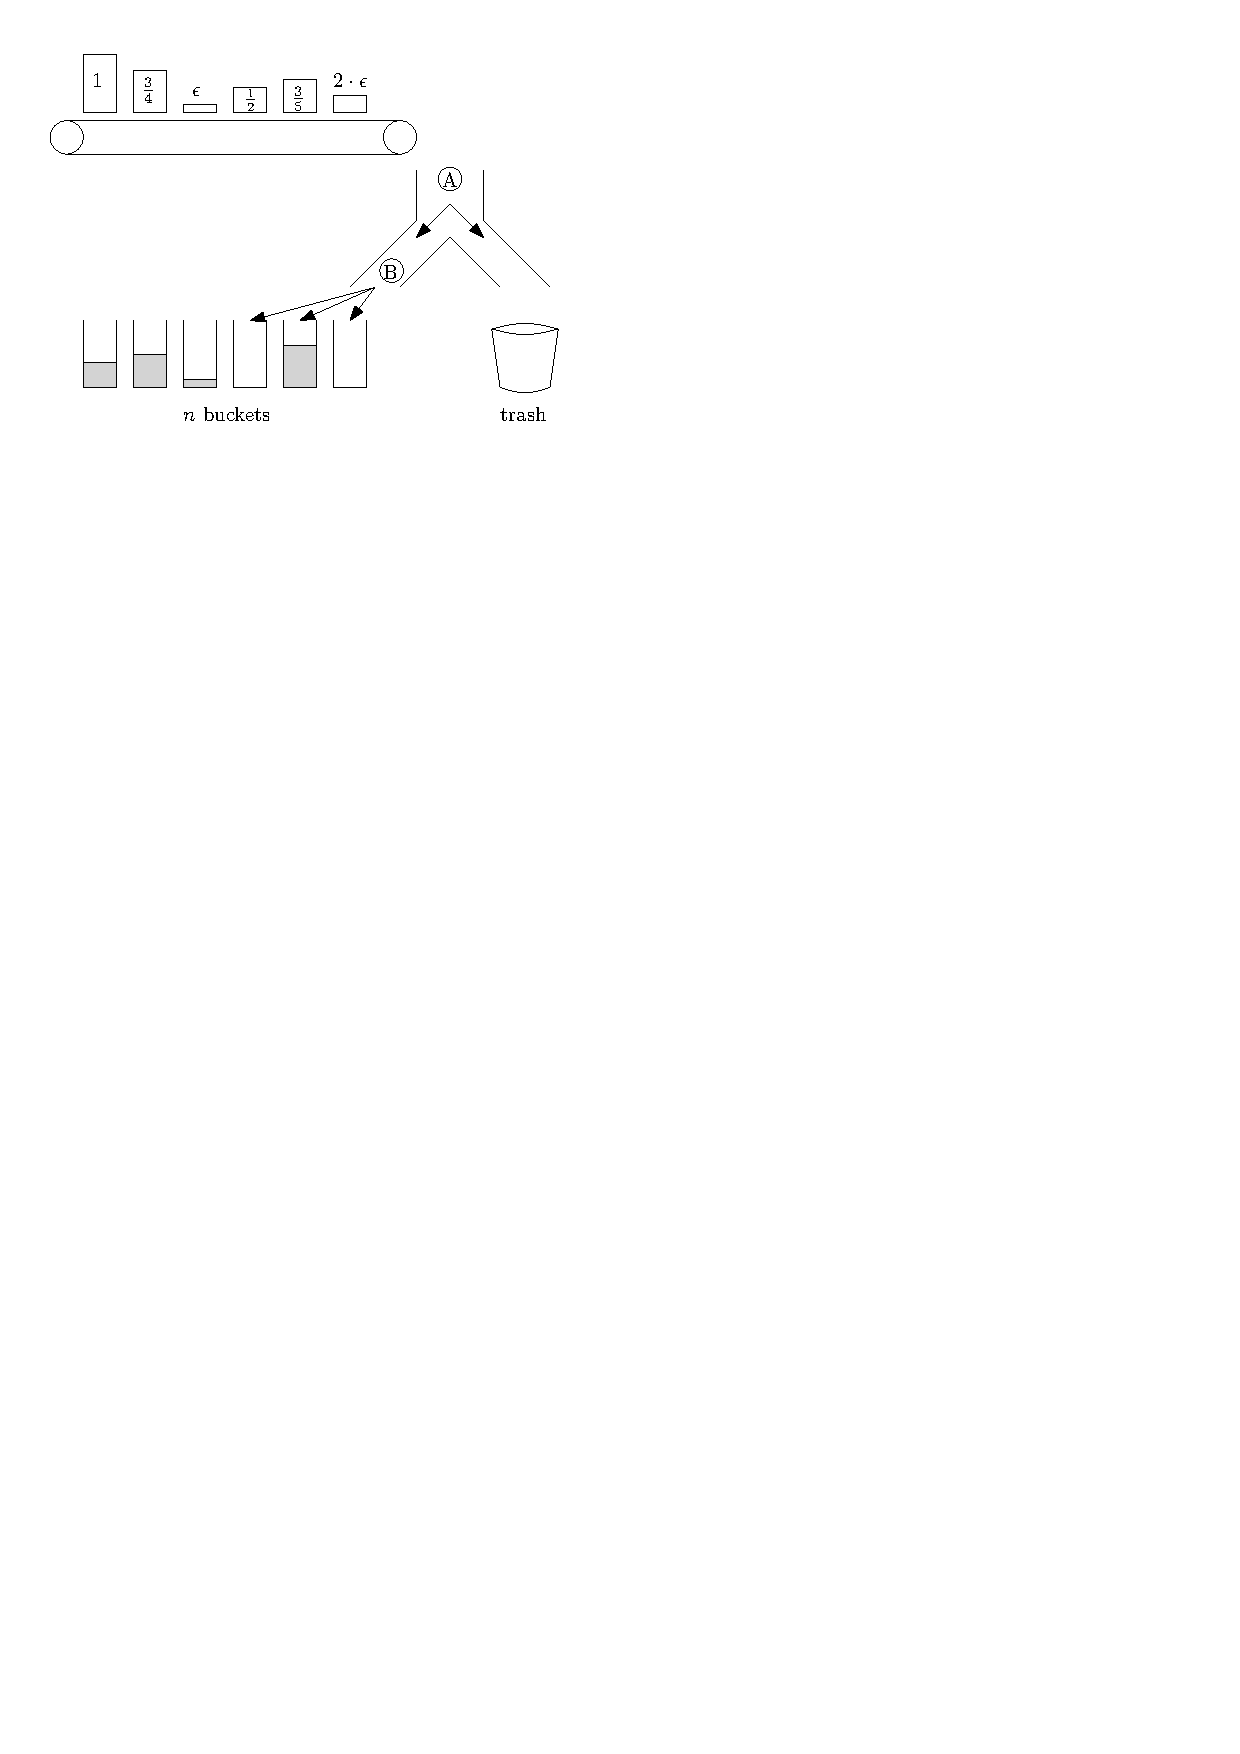
\includegraphics{figs/problem_formulation.pdf}
  
   \tiny $n$ kubełków o pojemności $1$, sekwencja przedmiotów w trybie online, nie usuwamy ani nie przenosimy
\end{frame}


\begin{frame}{Wariant Non-removable Proportional Online Knapsack}
  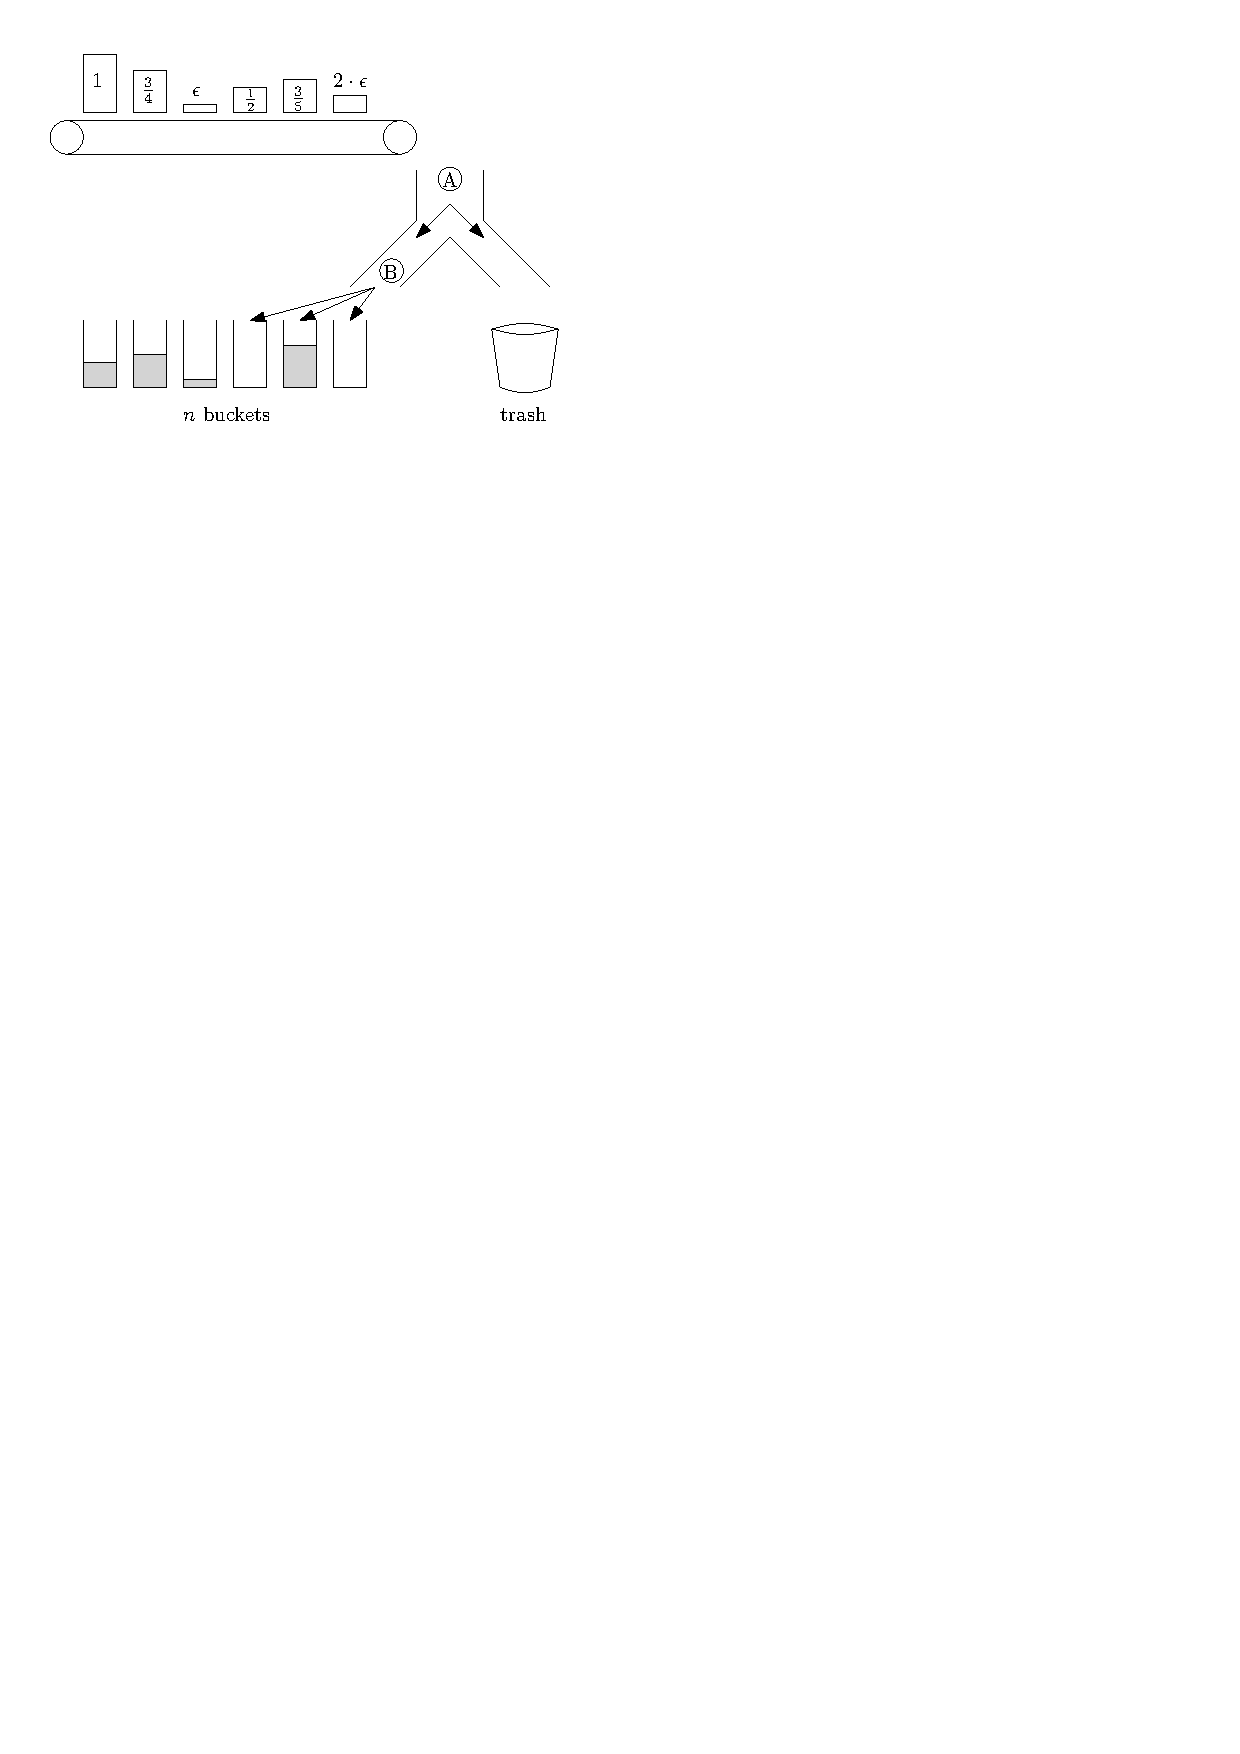
\includegraphics{figs/problem_formulation.pdf}
  \begin{enumerate}
    \item maksymalizacja sumy rozmiarów przyjętych przedmiotów
    \item konkurencyjność: $\frac{ALG}{OPT_{OFF}}$
  \end{enumerate}
\end{frame}


\begin{frame}{Wariant Non-removable Proportional Online Knapsack}
  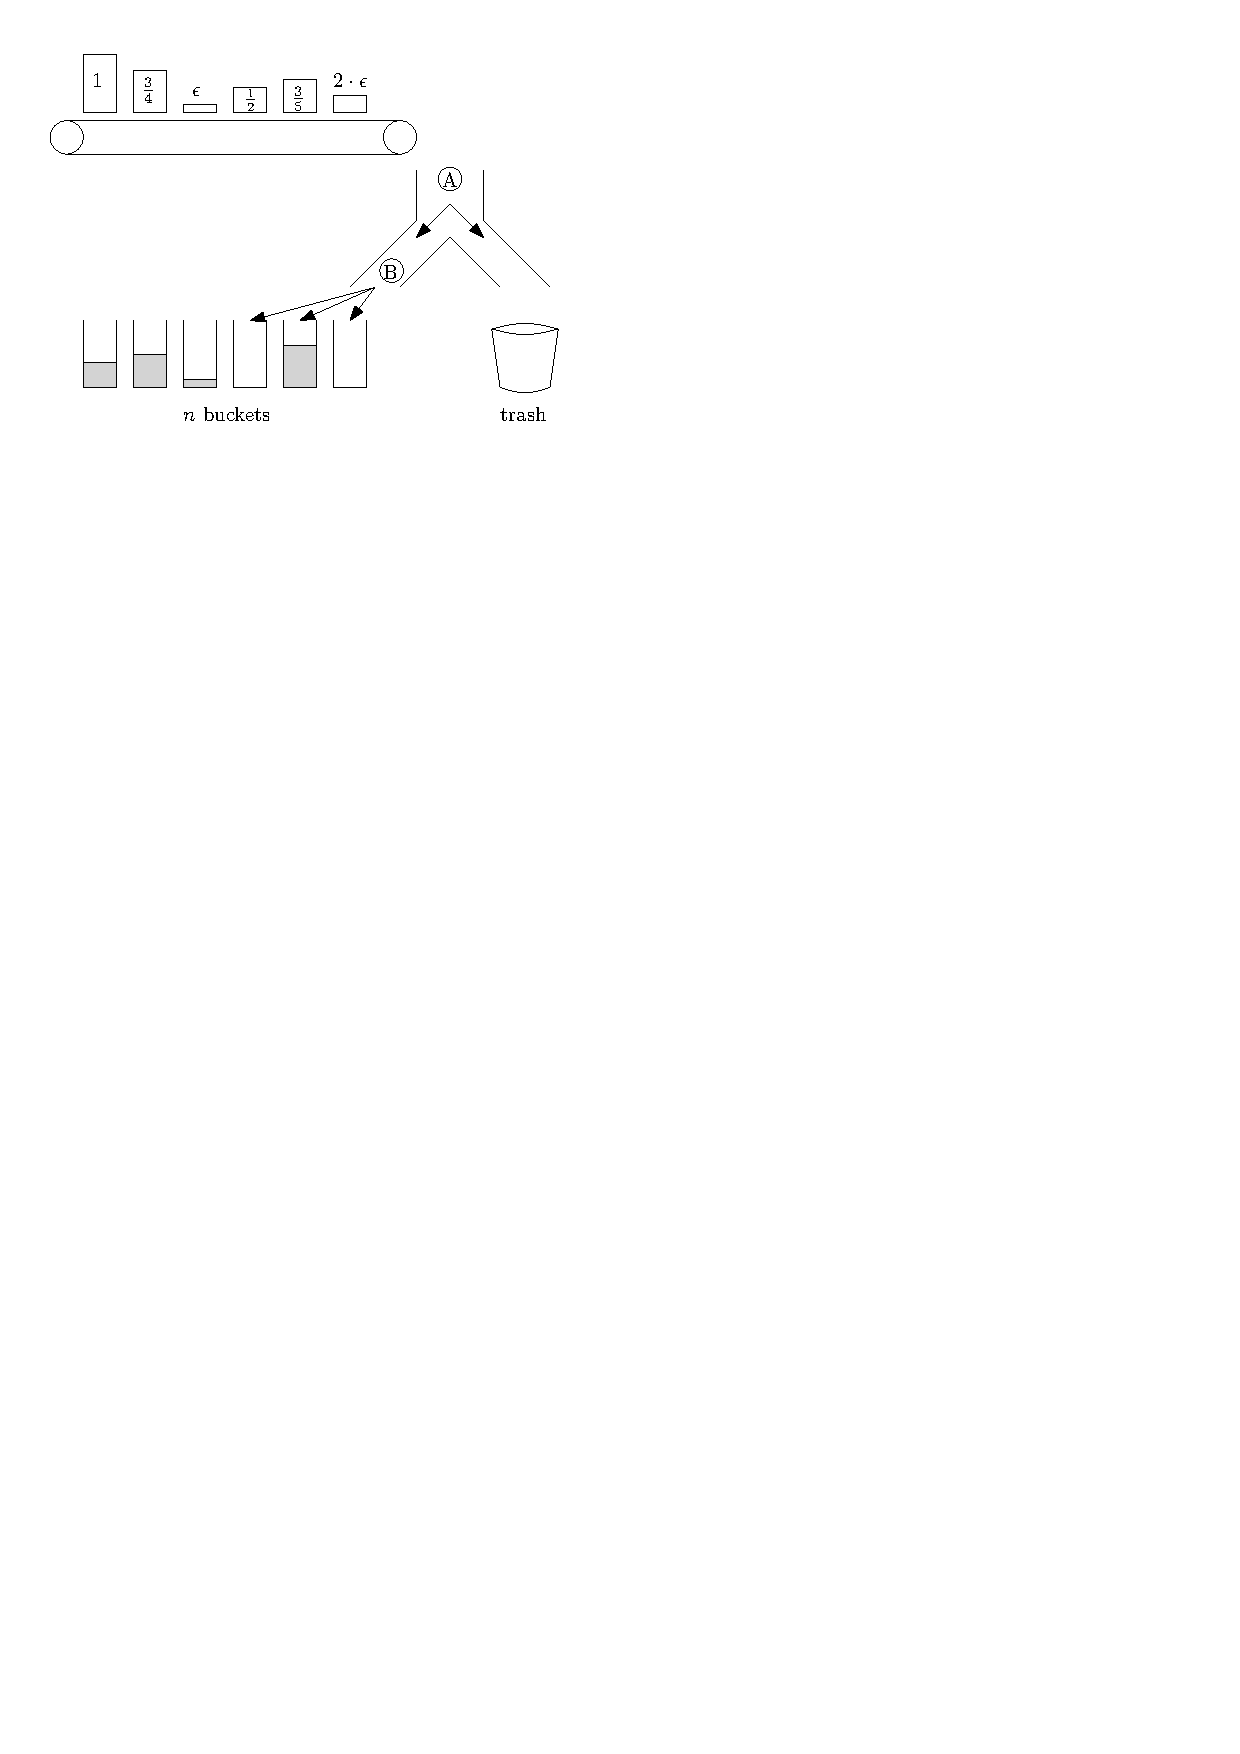
\includegraphics{figs/problem_formulation.pdf}
  \begin{enumerate}
    \item Greedy FirstFit jest $1/2$-konkurencyjny
    \item Górna granica konkurencyjności dla dowolnego algorytmu zrandomizowanego: $R = 1/(1+\ln(2)) \approx 0.59$
  \end{enumerate}
\end{frame}


\begin{frame}{Poprzednie rezultaty (Łukasz Jeż, Marek Cygan)}
  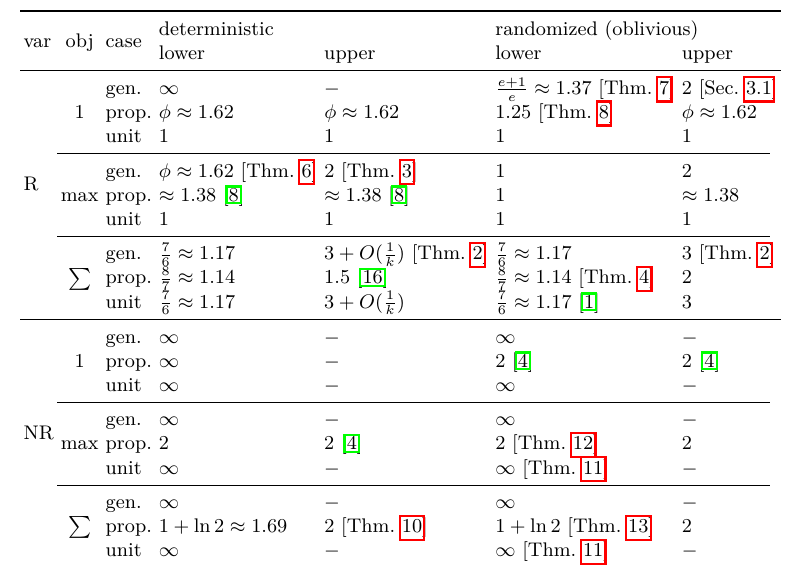
\includegraphics[width=0.9\textwidth]{figs/jez-cygan.png}
\end{frame}


\begin{frame}{Temat dzisiejszej prezentacji}
  Notacja:
  \begin{enumerate}
    \item Duże przedmioty: $(1/2, 1]$ -- mieszczą się po 1 w kubełku
    \item Średnie przedmioty: $(1/3, 1/2]$ -- mieszczą się po 2 w kubełku
  \end{enumerate}

  \vspace{1cm}
  
  Przedstawię dwa algorytmy:
  
  \begin{enumerate}
    \item Optymalny algorytm dla dużych przedmiotów
    \item Optymalny algorytm dla dużych i średnich przedmiotów
  \end{enumerate}
\end{frame}

\begin{frame}{Algorytm dla dużych przedmiotów $(1/2, 1]$}

\[
f(x) =
\begin{cases}
  1/2 &\mbox{if } x \leq R \enspace, \\
  (2e)^{x-1} & \textnormal{otherwise.}
\end{cases}
\]


  
  \begin{algorithm}[H]
  When new item of size $s$ arrives:\\
  b := number of filled buckets \\
  \If{b = n}{ terminate } \If{$s \leq f((b+1)/n)$}{ reject } \Else{
    put item into any empty bucket }
  \caption{$\ALG_L$}
\end{algorithm}
\end{frame}


\begin{frame}{Wykres funkcji $f$}
  \[
f(x) =
\begin{cases}
  1/2 &\mbox{if } x \leq R \enspace, \\
  (2e)^{x-1} & \textnormal{otherwise.}
\end{cases}
\]


  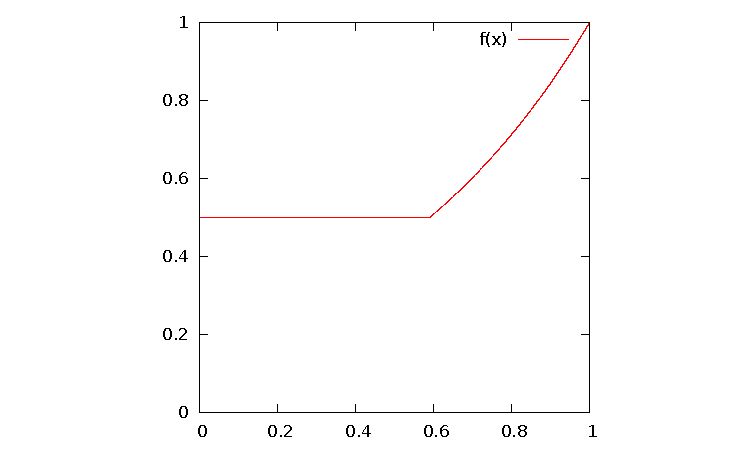
\includegraphics[width=0.9\textwidth]{figs/f.pdf}
\end{frame}

\begin{frame}{Zobrazowanie kubełków i funkcji progowej}
  \begin{center}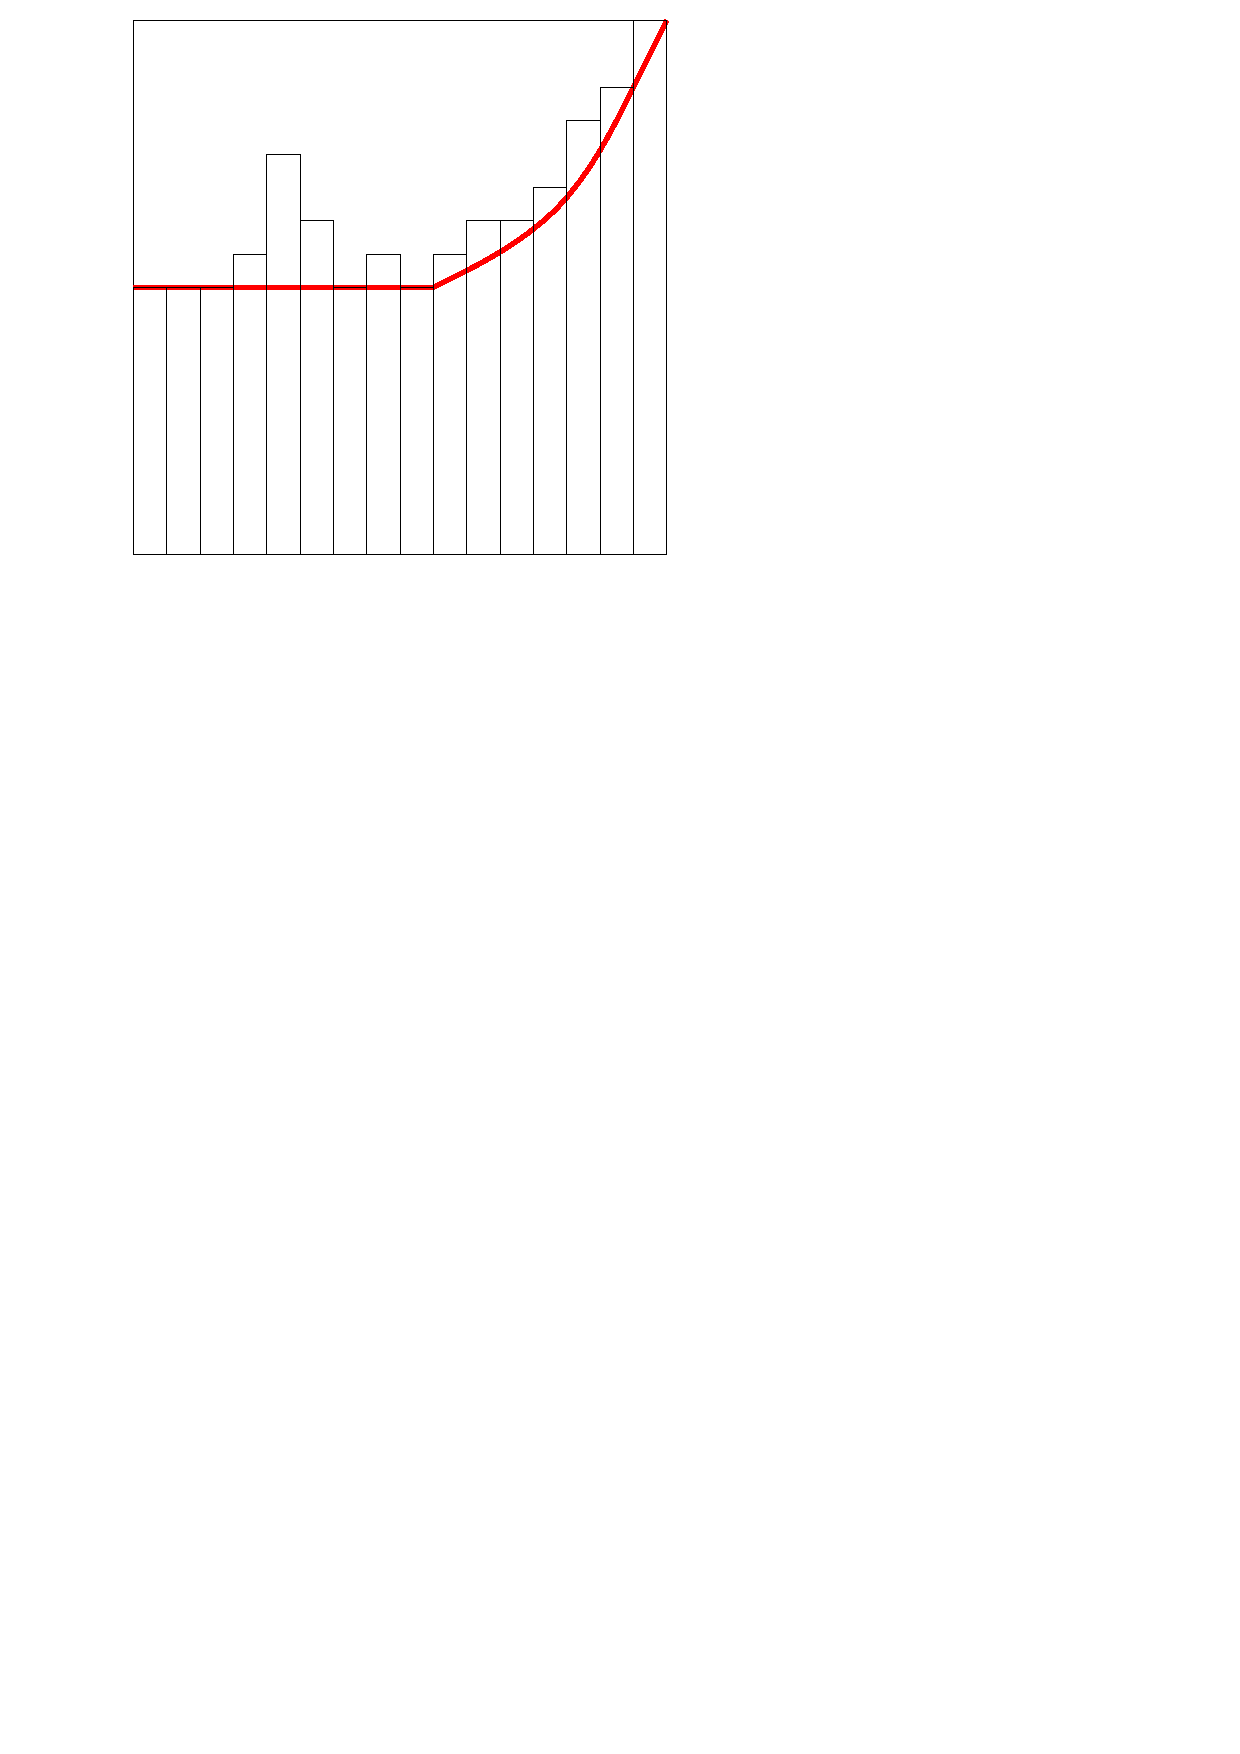
\includegraphics[width=0.4\textwidth]{figs/example1.pdf}\end{center}
  
  \begin{enumerate}
    \item Próg dla nowego przedmiotu zależy od liczby przyjętych przedmiotów (nie od ich rozmiarów)
    \item (metakomentarz) Stajemy się bardziej konserwatywni gdy mamy mniej zasobów
  \end{enumerate}
\end{frame}

\begin{frame}{Analiza algorytmu dla dużych przedmiotów $(1/2, 1]$}
  \begin{center}
    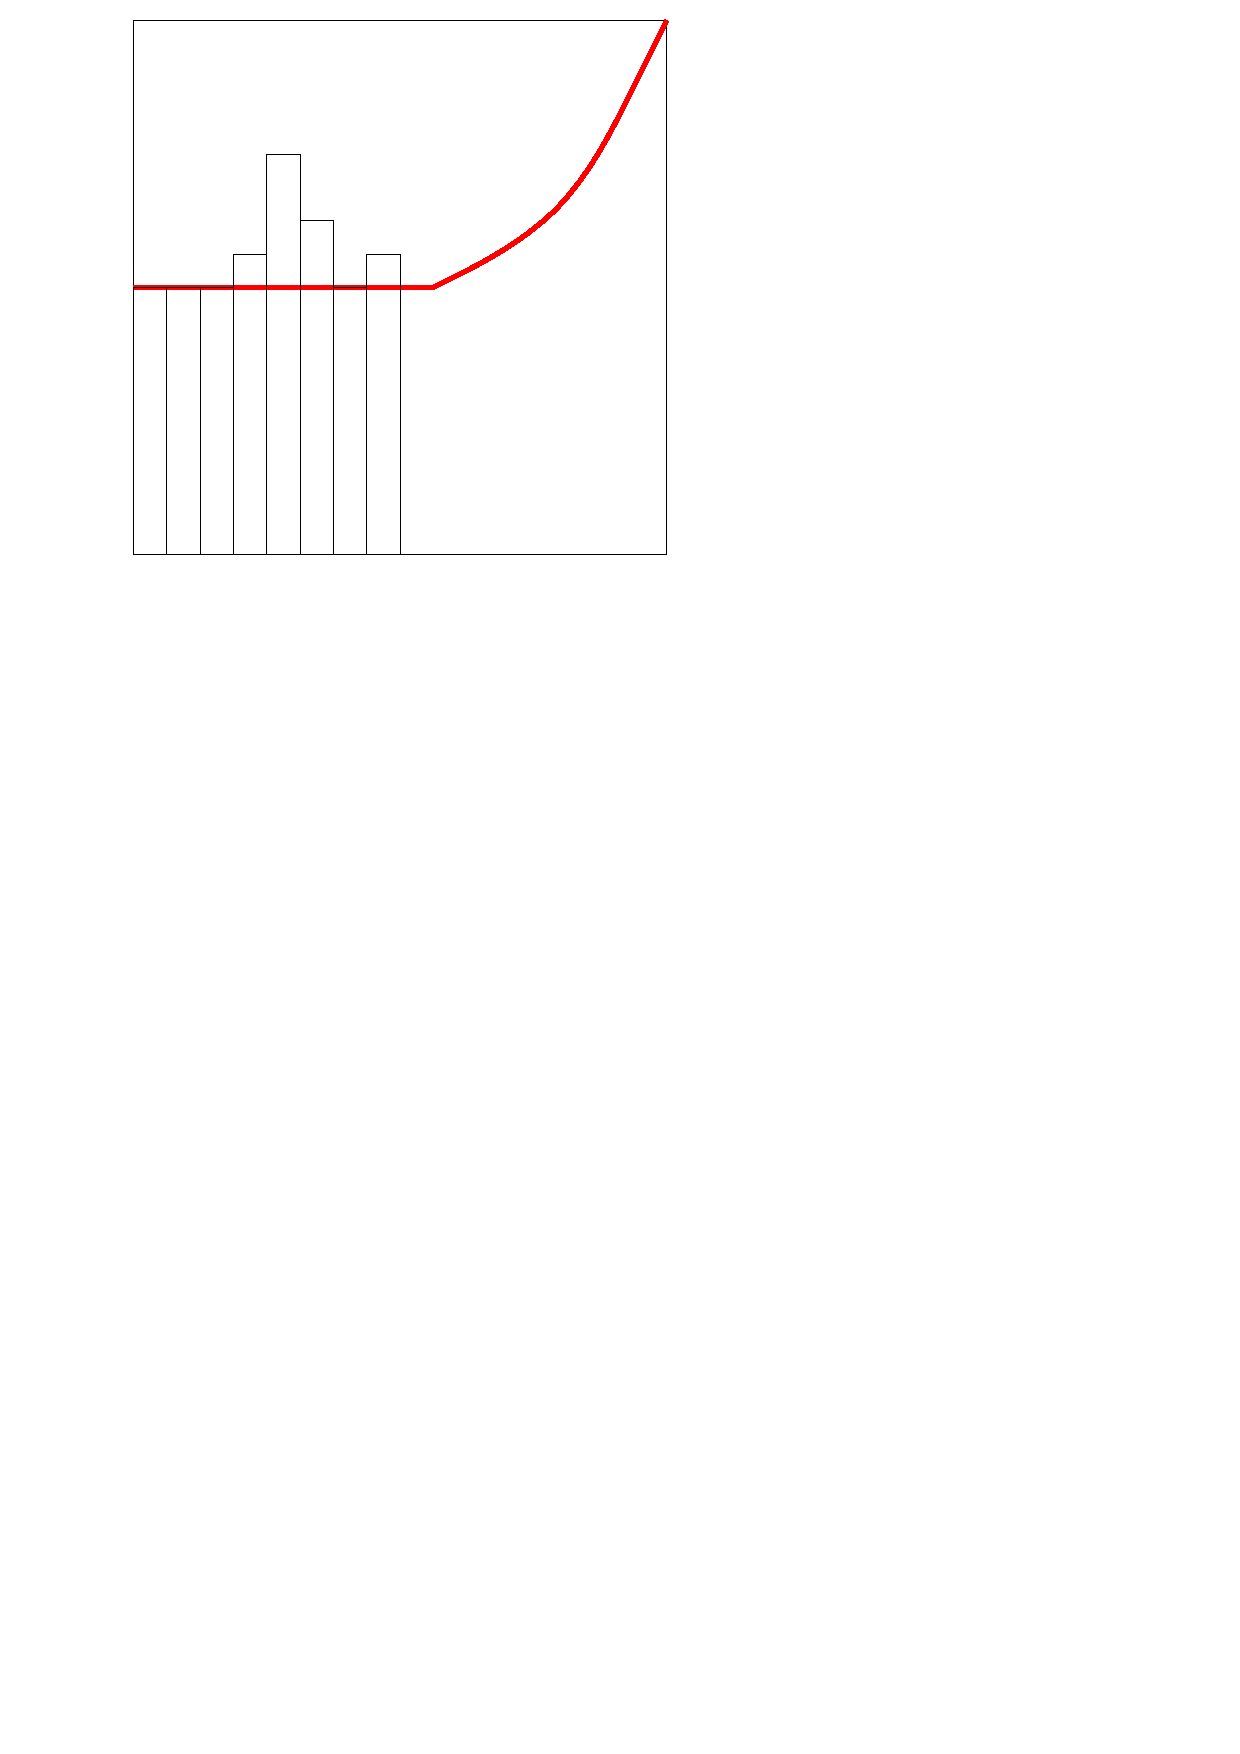
\includegraphics[width=0.6\textwidth]{figs/analysis_leqR.pdf}
  \end{center}

  \vspace{-0.1cm}
  
  Jeśli algorytm zakończył się zapełniając mniej niż $R\cdot n$ kubełków to zaakceptowaliśmy wszystko i jesteśmy optymalni
  \end{frame}

\begin{frame}{Analiza algorytmu dla dużych przedmiotów $(1/2, 1]$}
  \begin{center}
    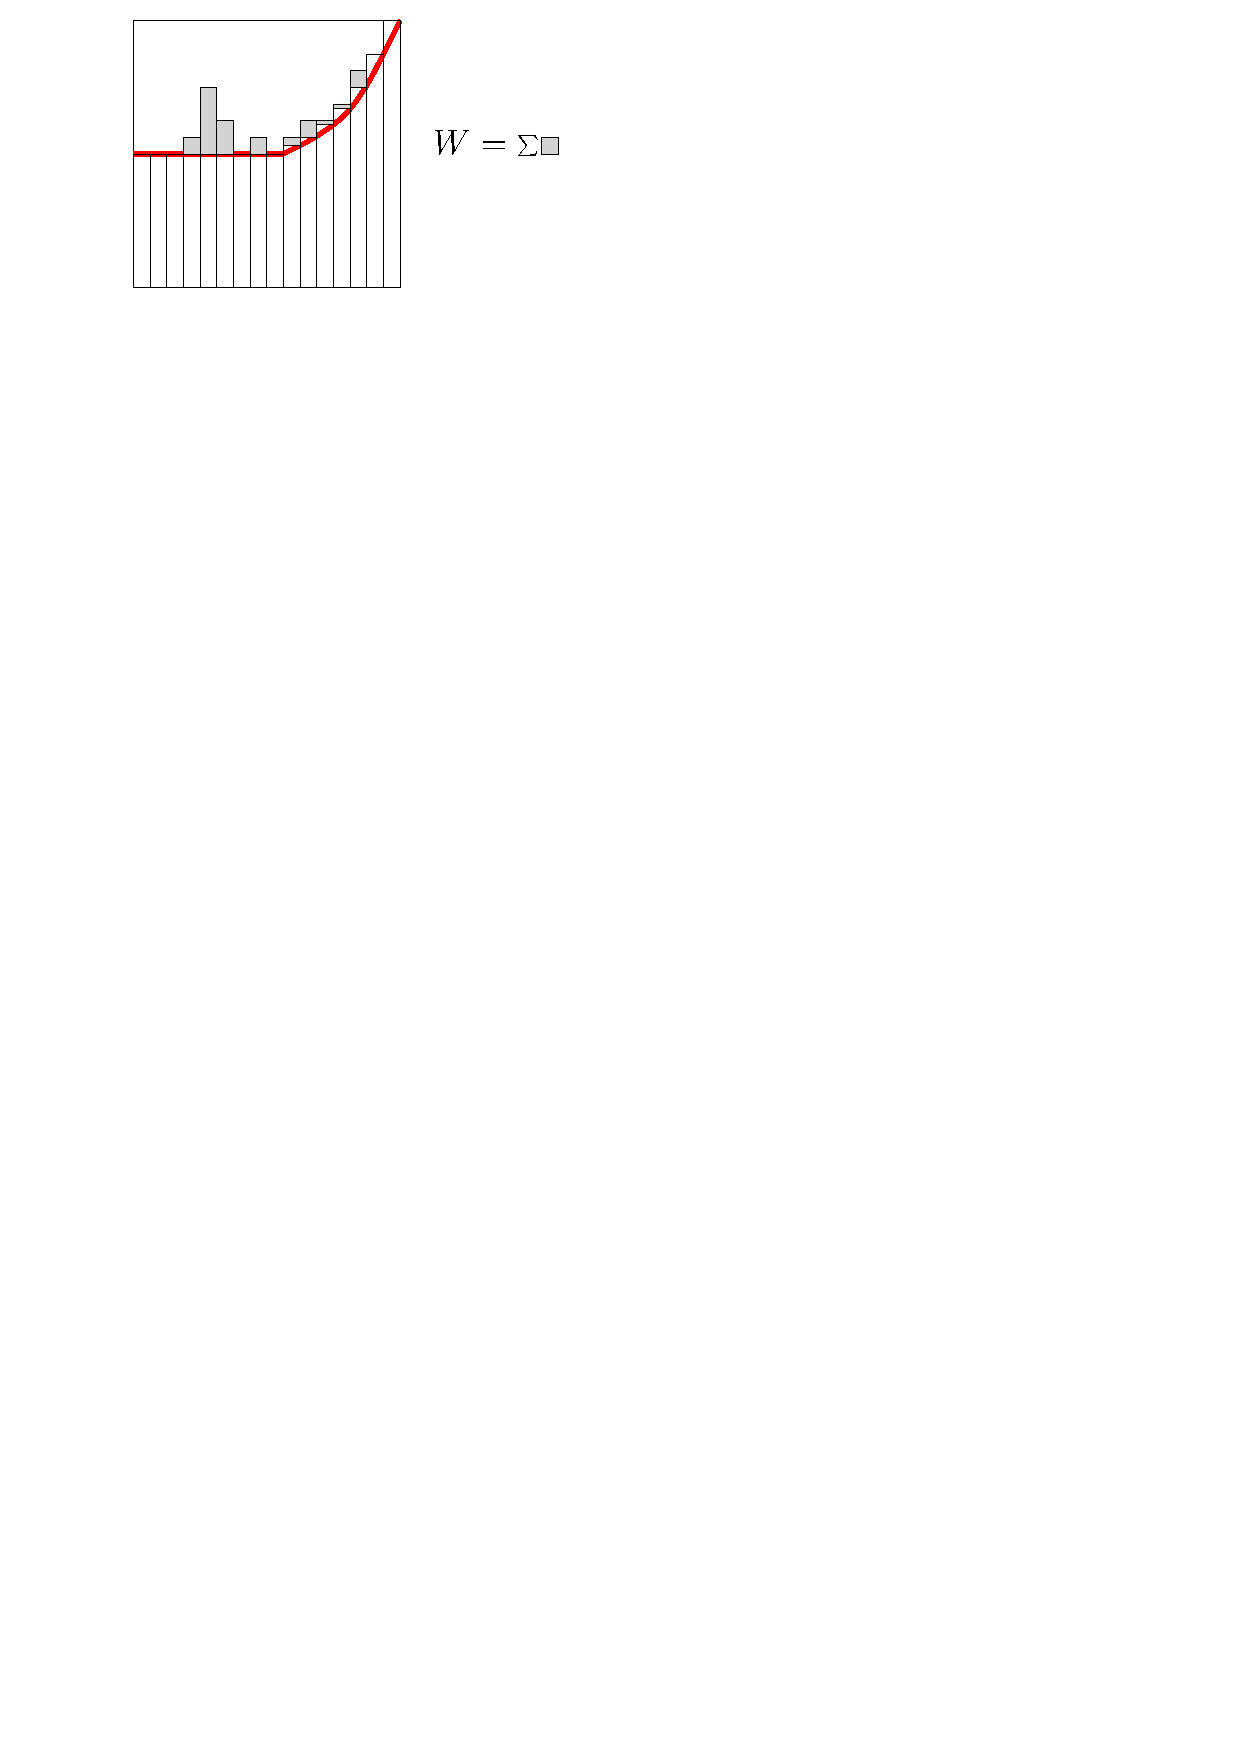
\includegraphics[width=0.6\textwidth]{figs/example2.pdf}
  \end{center}

  \vspace{-0.1cm}
  
  Jeśli algorytm zakończył zapełniając $b \geq R\cdot n$ kubełków to:
    \begin{itemize}
      \item adwersarz ``zostawia OPTowi na koniec'' przedmioty poniżej progu akceptacji $f(b)$
      \item $OPT \leq n\cdot f(b) + W$
      \item $ALG \geq n\cdot \int^{b}f(x) dx + W$
    \end{itemize}
\end{frame}

\begin{frame}{Pewna własność $f$}
  
  $$\forall_{b \in (R, 1]}\frac{{\color{red} \int^bf(x)dx}}{{\color{teal} f(b)}} = R$$
  
  \begin{center}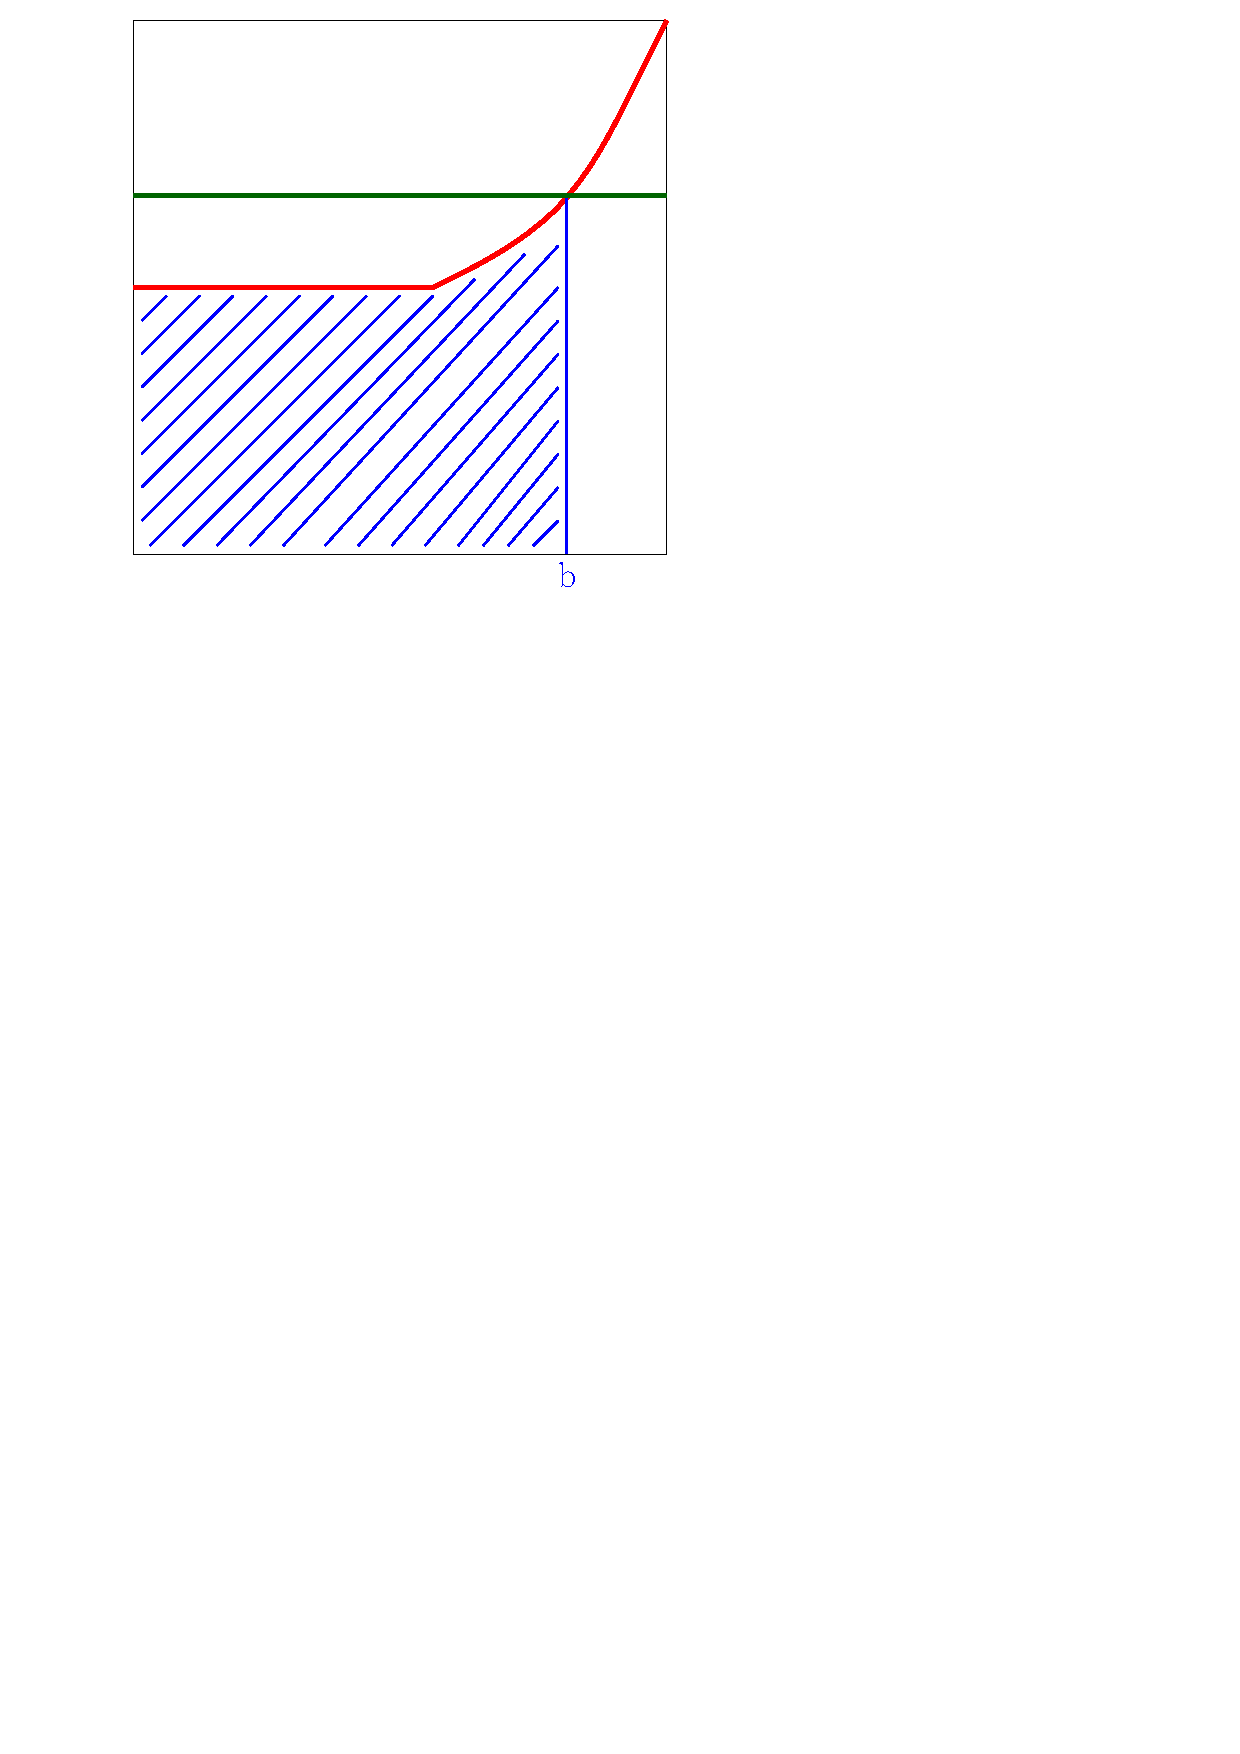
\includegraphics[width=0.35\textwidth]{figs/f_properties}\end{center}

  $$ \Rightarrow \frac{ALG}{OPT} \geq \frac{\int^bf(x)dx + W}{f(b) + W} \geq R $$
\end{frame}


\begin{frame}{Rozgrzewka -- wszystkie średnie przedmioty mają tę samą wielkość}
  Algorytm dla dużych przedmiotów $(1/2, 1]$ i średnich przedmiotów o jednym, ustalonym rozmiarze $s$:
  
  \begin{enumerate}
    \item Traktujemy duże przedmioty jak Algorytm dla dużych przedmiotów
    \item Akceptujemy wszystkie średnie przedmioty
    \item Decyzja do podjęcia: średnie po 1 czy po 2 w kubełku? Odpowiedź: utrzymuj pewną frakcję (wszystkich kubełków) pojedynczych a po przekroczeniu progu: podwójne
    \item Jeśli możemy to łączymy duże i średnie przedmioty
  \end{enumerate}
\end{frame}


\begin{frame}{Rozgrzewka -- wszystkie średnie przedmioty mają tę samą wielkość}

  \begin{center}
    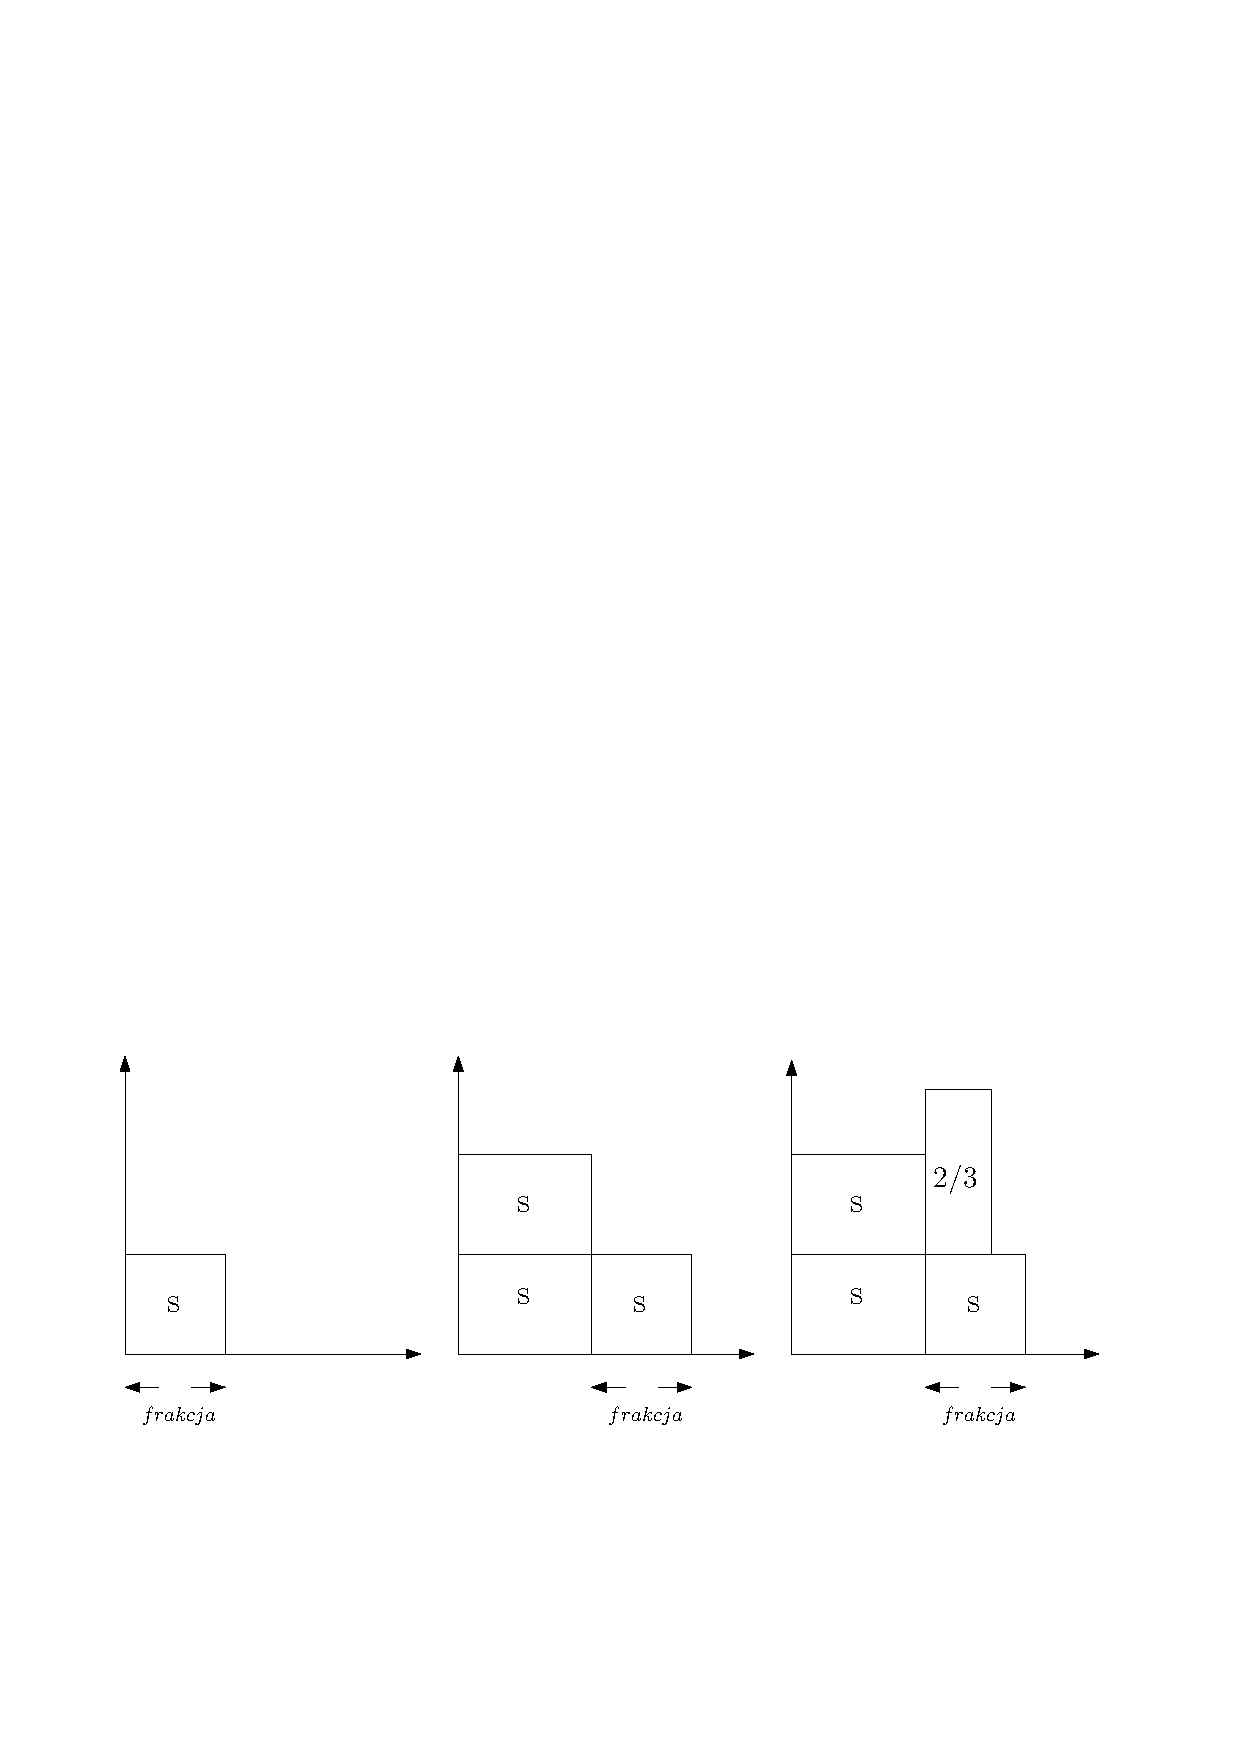
\includegraphics[width=0.7\textwidth]{figs/fraction.pdf}
  \end{center}
  
  \begin{enumerate}
    \item Utrzymuj pewną frakcję (wszystkich kubełków) pojedynczych a po przekroczeniu progu: podwójne
    \item Jeśli możemy to łączymy duże i średnie przedmioty
  \end{enumerate}
\end{frame}

\begin{frame}{Analiza algorytmu -- przypadek gdy zostały puste kubełki}
  Korzystamy z dwóch własności algorytmu:
  \begin{enumerate}
    \item Traktujemy duże przedmioty jak Algorytm 1
    \item Akceptujemy wszystkie średnie przedmioty
  \end{enumerate}


  Szacujemy zysk OPTa i Algorytmu 2:
  
  \begin{enumerate}
  \item $ALG(I) = ALG_L(I_L) + weight(I_M)$
  \item $OPT(I) \leq OPT(I_L) + OPT(I_M) \leq OPT(I_L)+weight(I_M)$
  \end{enumerate}

  Sprowadzamy analizę Algorytmu 2 do analizy Algorytmu 1:
  
   $$ \frac{ALG(I)}{OPT(I)} \geq \frac{ALG_L(I_L) + weight(I_M)}{OPT(I_L) +weight(I_M)} \geq \frac{ALG_L(I_L)}{OPT(I_L)}$$
\end{frame}

\begin{frame}{Analiza algorytmu -- przypadek, gdy wszystkie kubełki zajęte}
  \begin{center}
    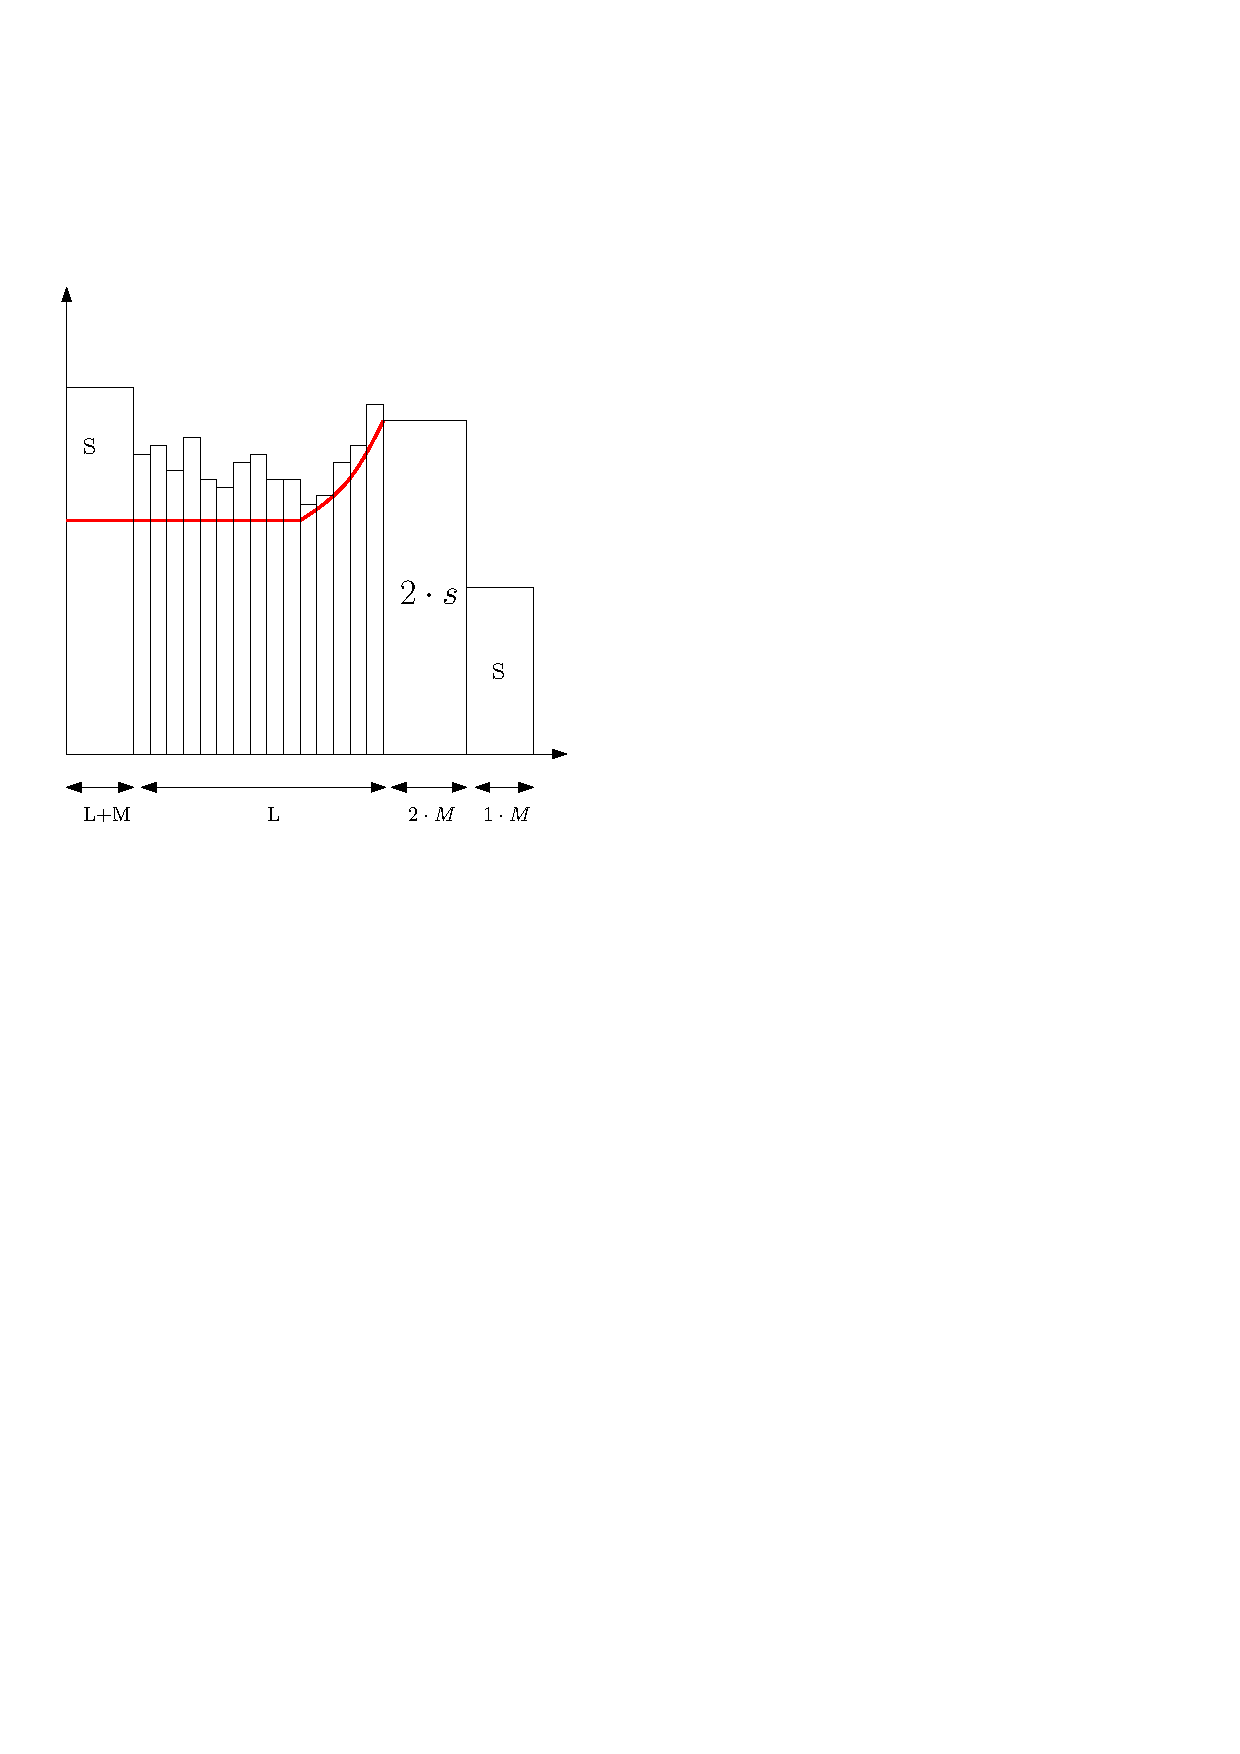
\includegraphics[width=0.5\textwidth]{figs/classes.pdf}
    \end{center}

  \begin{enumerate}
    \item Rozpatrujemy sytuację po zakończeniu działania algorytmu
    \item Szacujemy zysk na każdej klasie kubełków
    \item Dwa podprzypadki: istnieje klasa $1M$ i nie istnieje
  \end{enumerate}
\end{frame}

\begin{frame}{Analiza algorytmu -- przypadek, gdy wszystkie kubełki zajęte}
  \begin{center}
    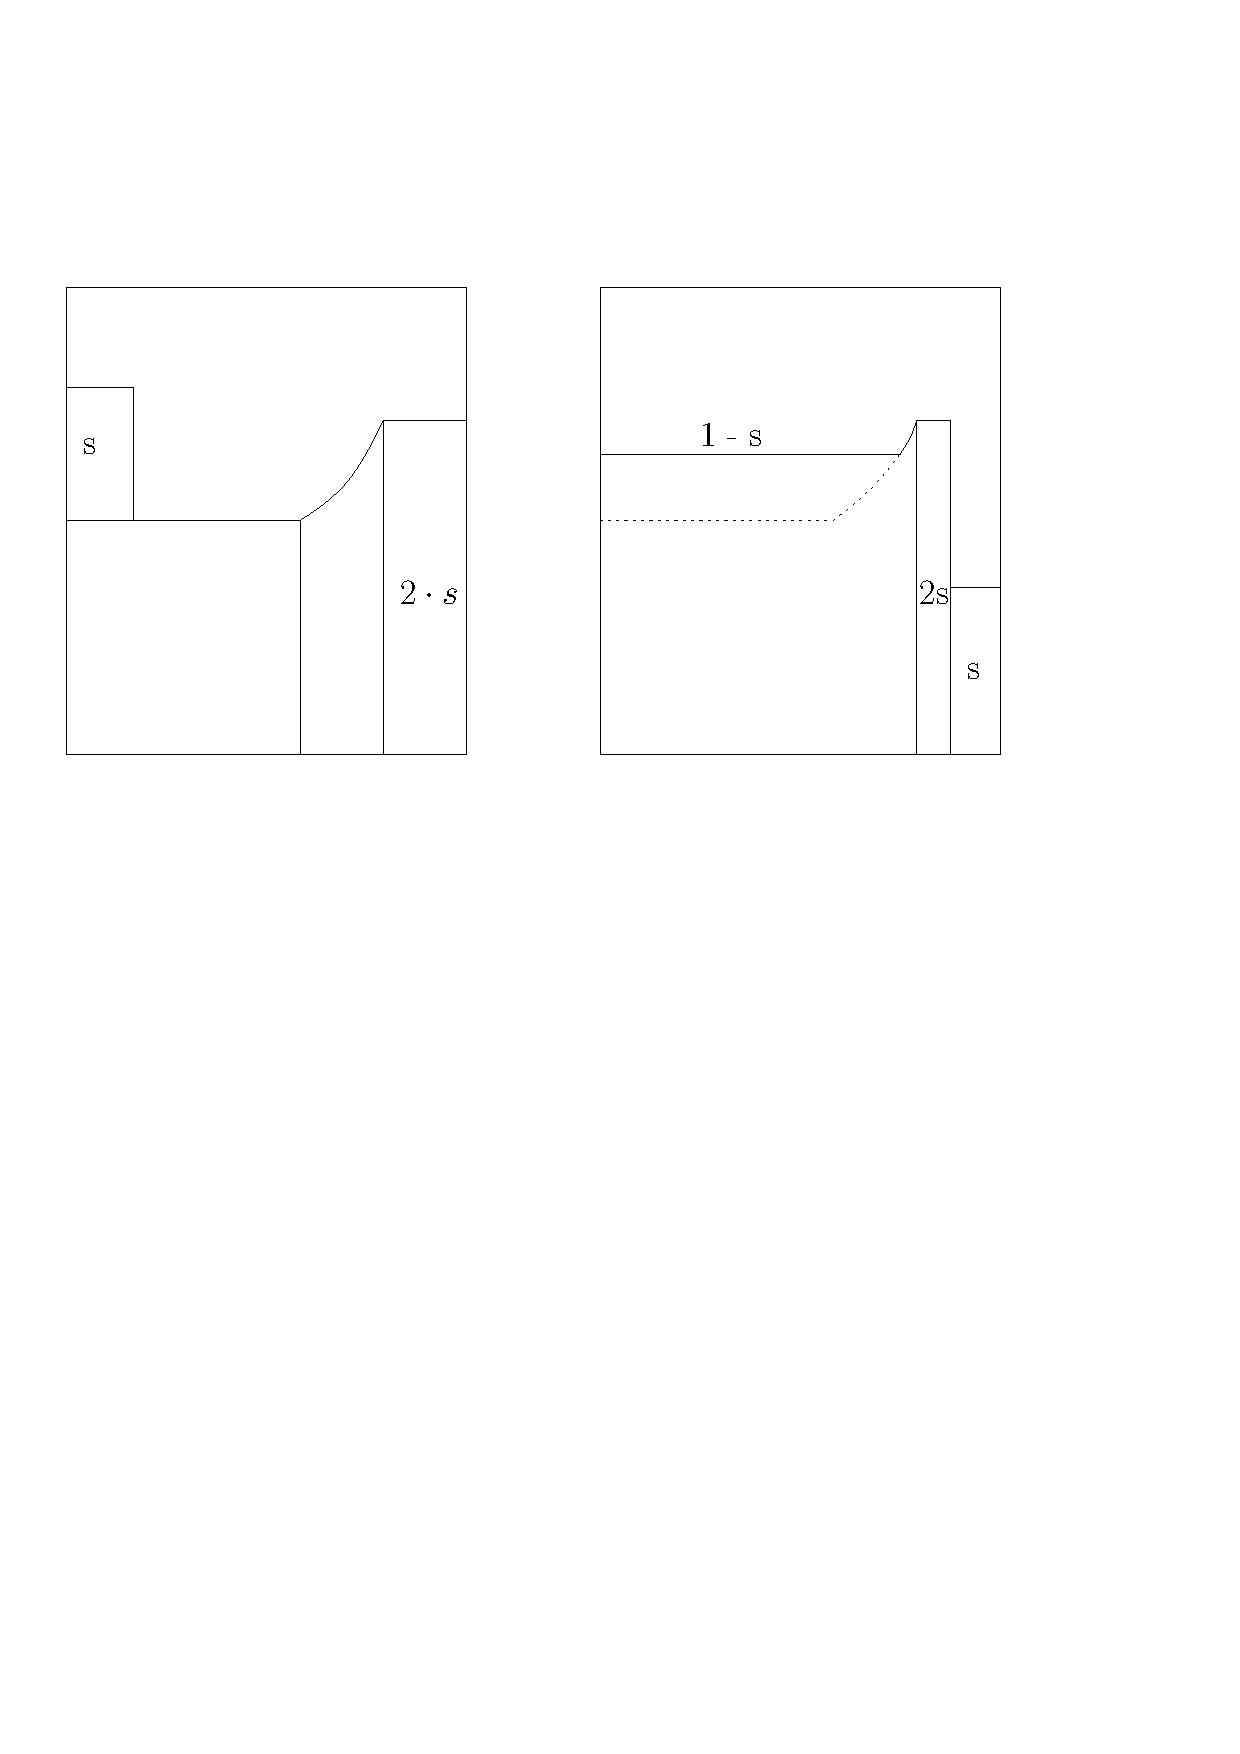
\includegraphics[width=0.7\textwidth]{figs/G1G2.pdf}
  \end{center}

    \begin{itemize}
      \item (po lewej) nie zostały kubełki pojedyncze -- były, ale zostały zjedzone przez duże
      \item (po prawej) zostały kubełki pojedyncze -- nie mogliśmy połączyć ich z dużymi, więc szacujemy duże przez $\max\{ f(b_i), 1 - s \}$
      \end{itemize}
\end{frame}

\begin{frame}{Analiza algorytmu -- dwa przypadki i ograniczenia na frakcję}
  \begin{center}
    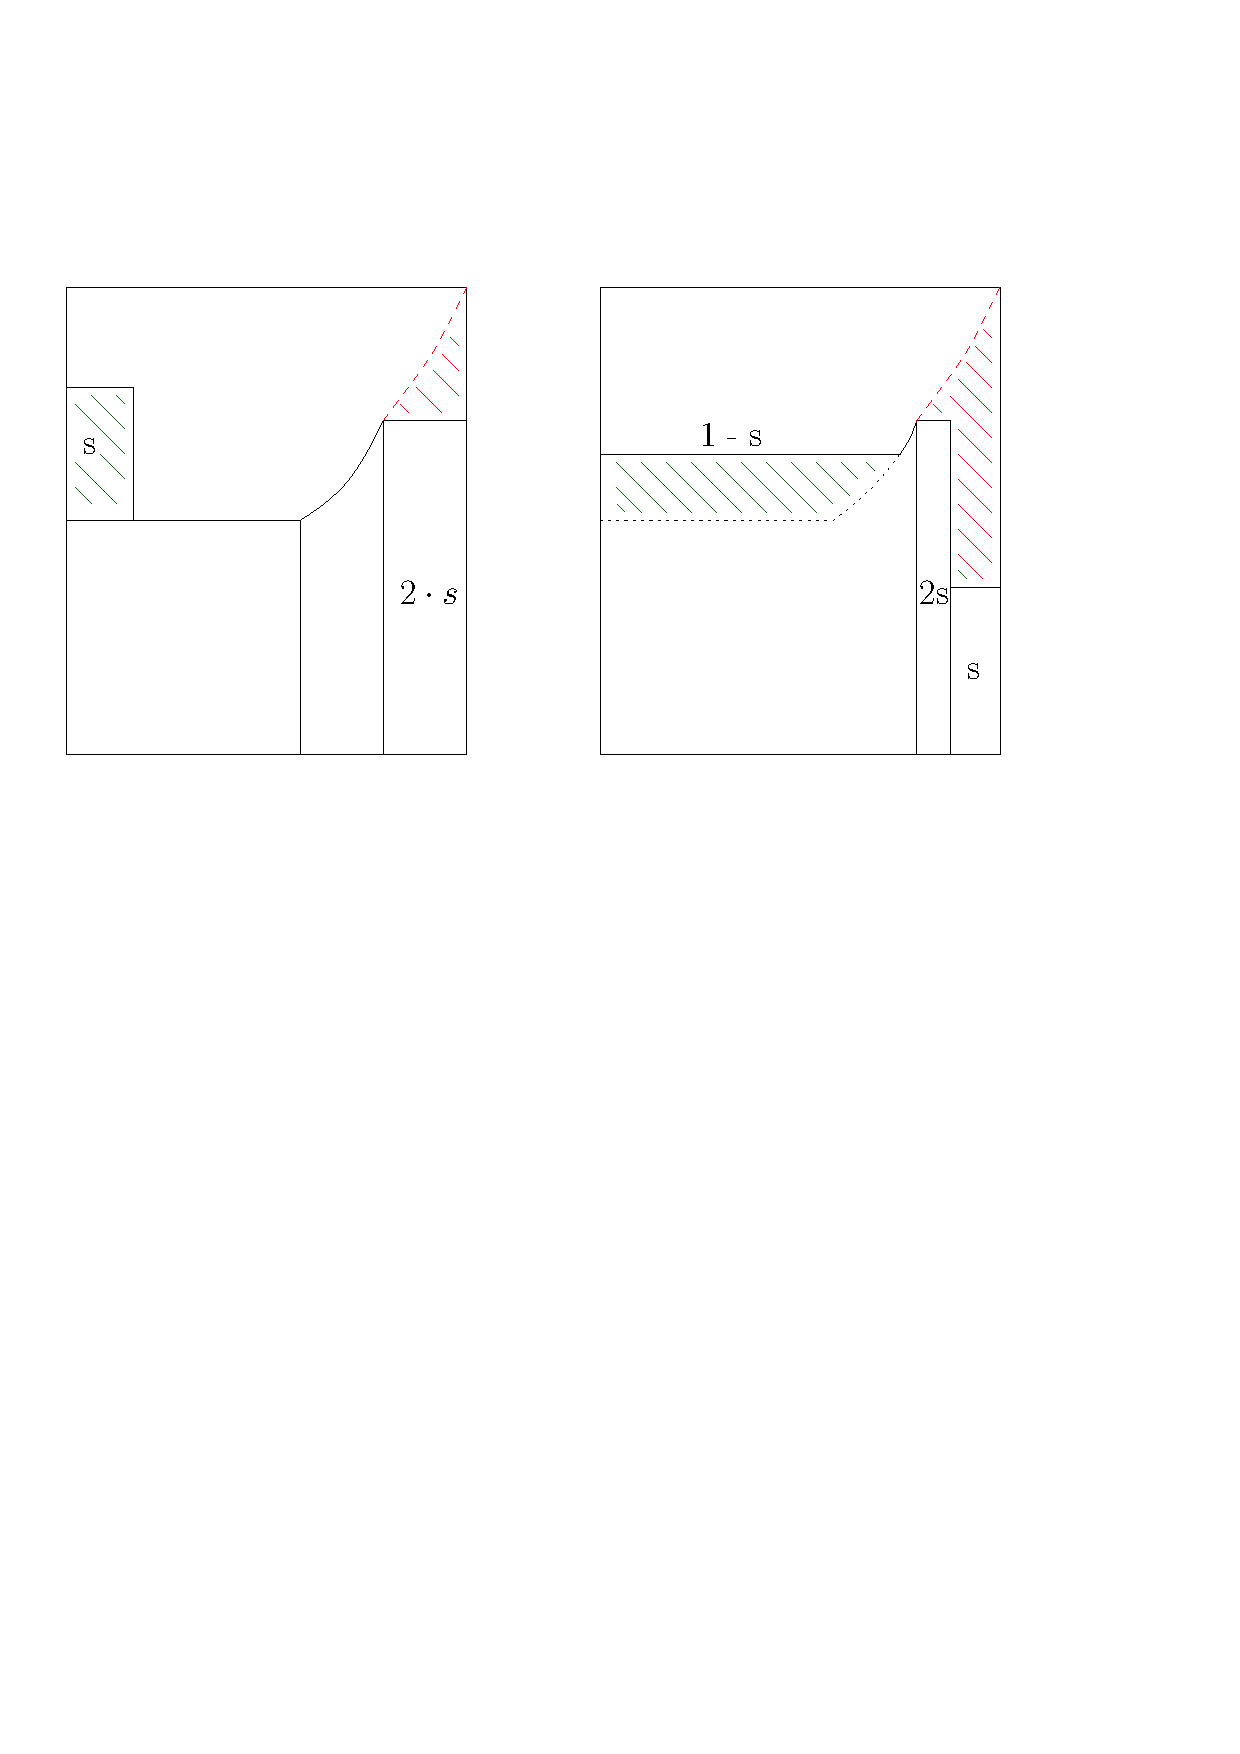
\includegraphics[width=0.9\textwidth]{figs/G1G2_insuff.pdf}
  \end{center}

  Po lewej: chcemy, żeby frakcja pojedynczych była jak największa. Po prawej: chcemy, żeby frakcja była jak najmniejsza.
\end{frame}


\begin{frame}{Analiza algorytmu -- dwa przypadki i ograniczenia na frakcję}
  \begin{center}
    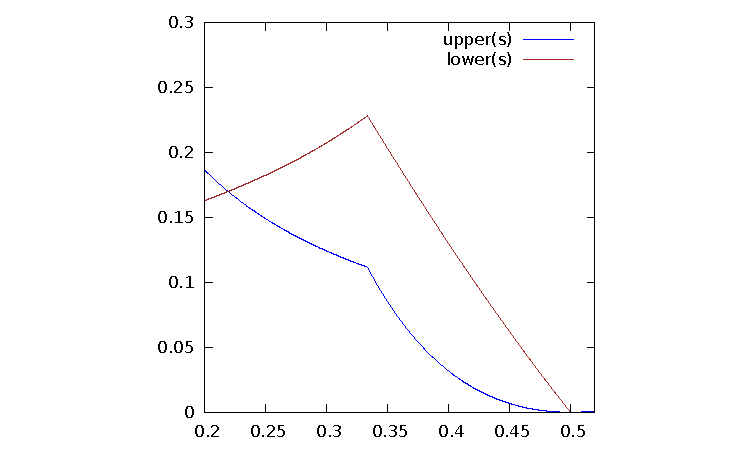
\includegraphics[width=0.8\textwidth]{figs/04.pdf}
  \end{center}

  \tiny Nieciągłość pochodnej w $1/3$ jest spowodowana faktem, że analizujemy wkładanie $2$ średnich przedmiotów do kubełka, a mniejsze przedmioty wchodzą po $3, 4, \ldots$.
\end{frame}

\begin{frame}{Więcej rozmiarów średnich przedmiotów}
  \footnotesize
  \begin{enumerate}
    \item  Definiujemy strukturę, w której trzymamy wszystkie średnie przedmioty POZA tymi po dwa średnie w kubełku.
    \item W strukturze są zarówno przedmioty pojedyncze jak i połączone z dużymi.
    \item Przedmioty mieszczą się w strukturze jeśli posortowane znajdują się pod wykresem funkcji $g$
    \item Funkcja $g^{-1}(s)$ określa, ile przedmiotów $\geq s$ utrzymujemy pojedynczo.
  Funkcja $g^{-1}$ musi zawierać się między ograniczeniami na frakcję.
  \end{enumerate}
  
  \begin{center}
    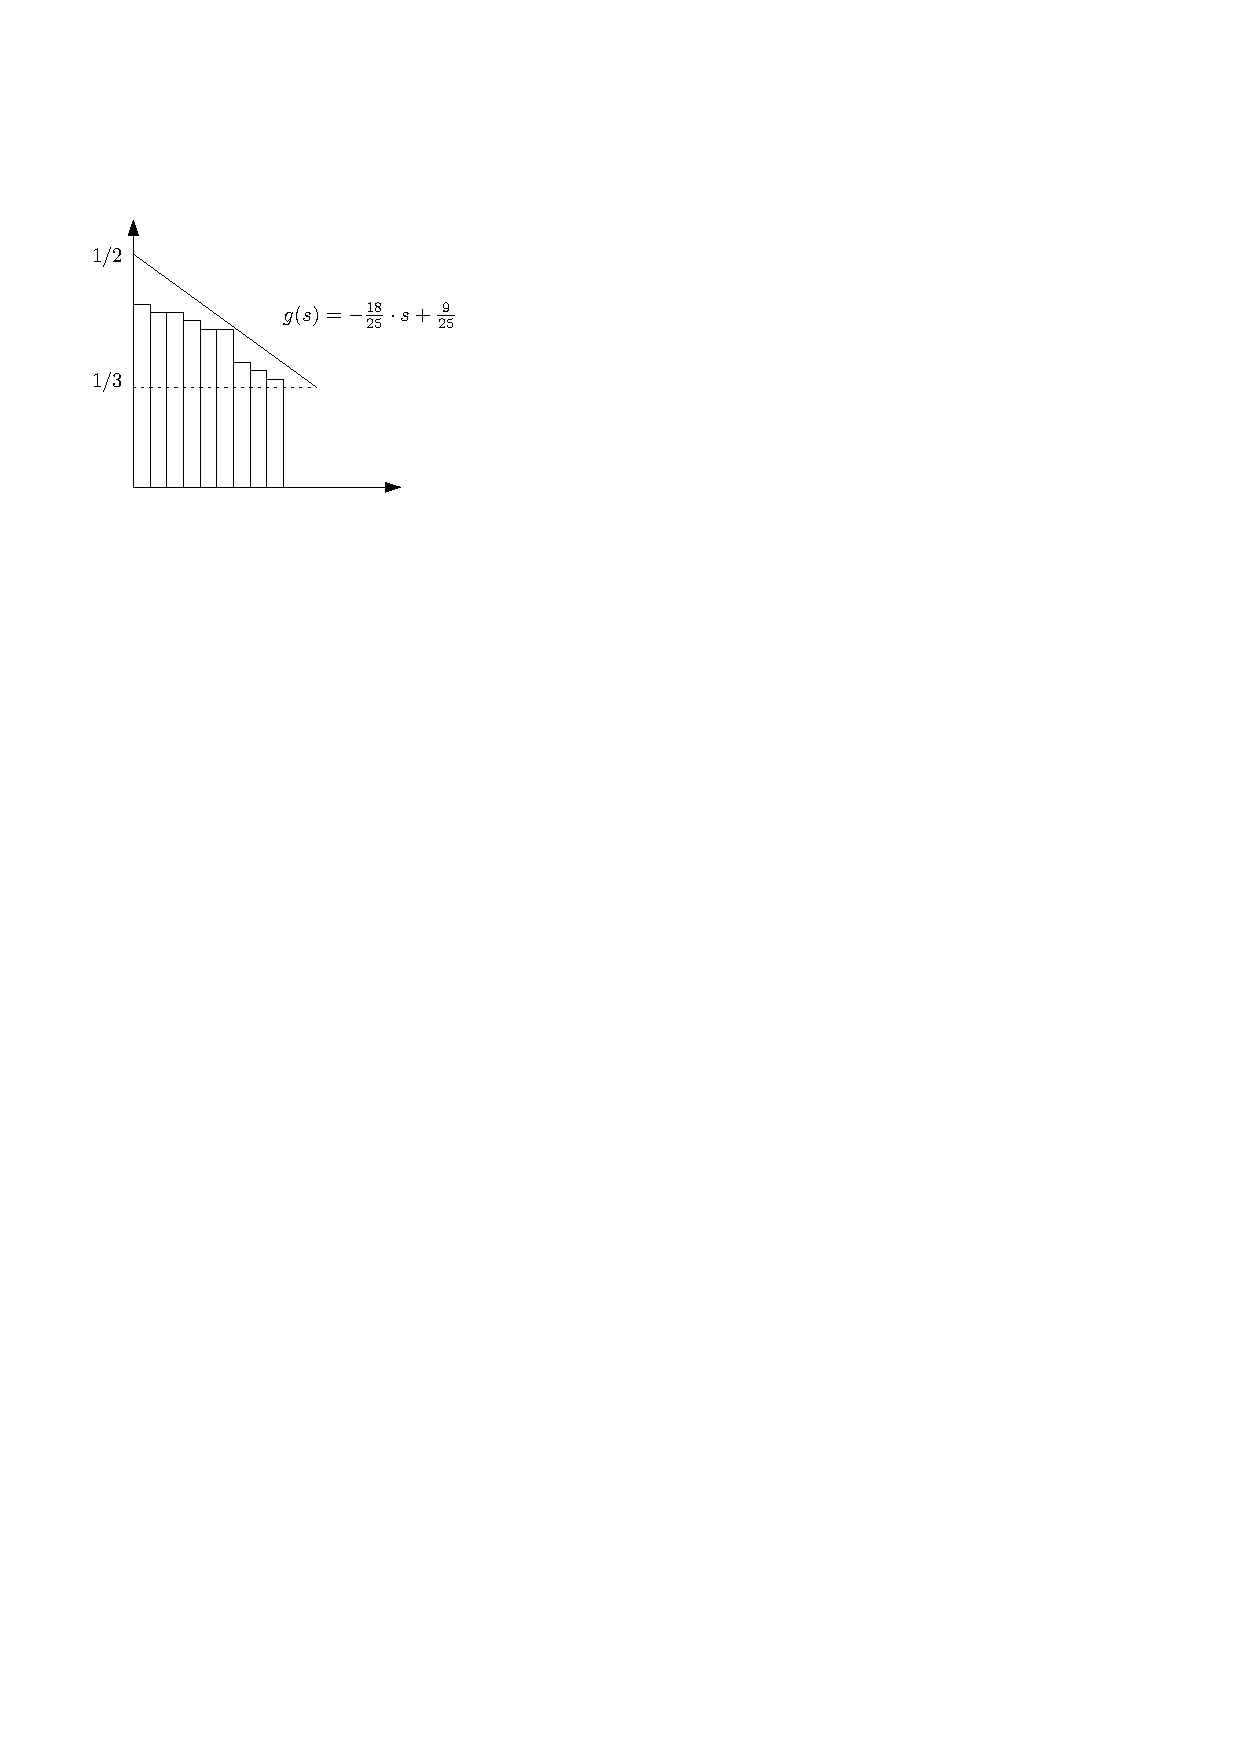
\includegraphics[width=0.5\textwidth]{figs/D.pdf}
  \end{center}


\end{frame}

\begin{frame}{Relacja minimalny ciasny-minimalny odrzucony ze struktury}
  Mówimy, że $t$ jest ciasny jeśli nie możemy dołożyć kolejnego przedmiotu o wielkości $t$ do struktury z powodu zbyt dużej liczby przedmiotów większych niż $t$. 
  \vspace{-0.5cm}
  \begin{center}
    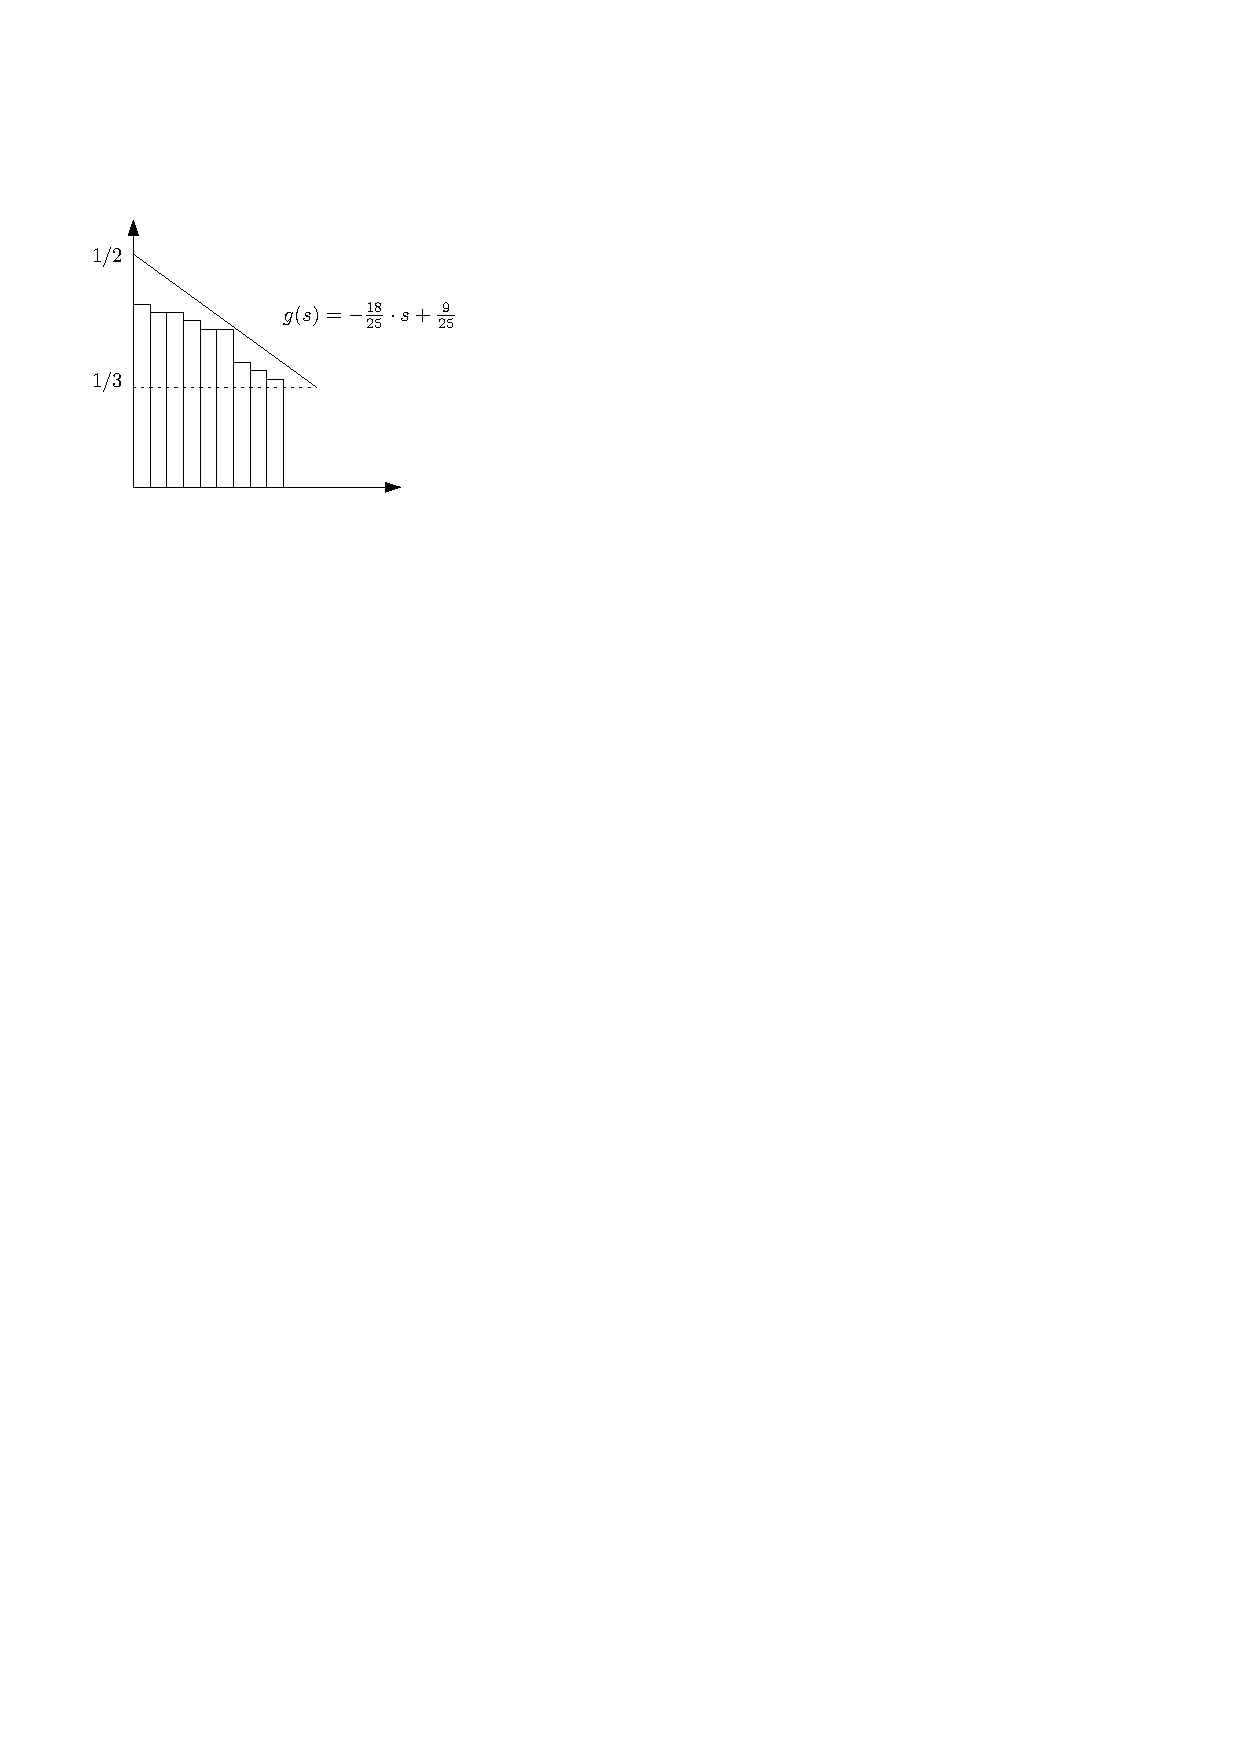
\includegraphics[width=0.5\textwidth]{figs/D.pdf}
    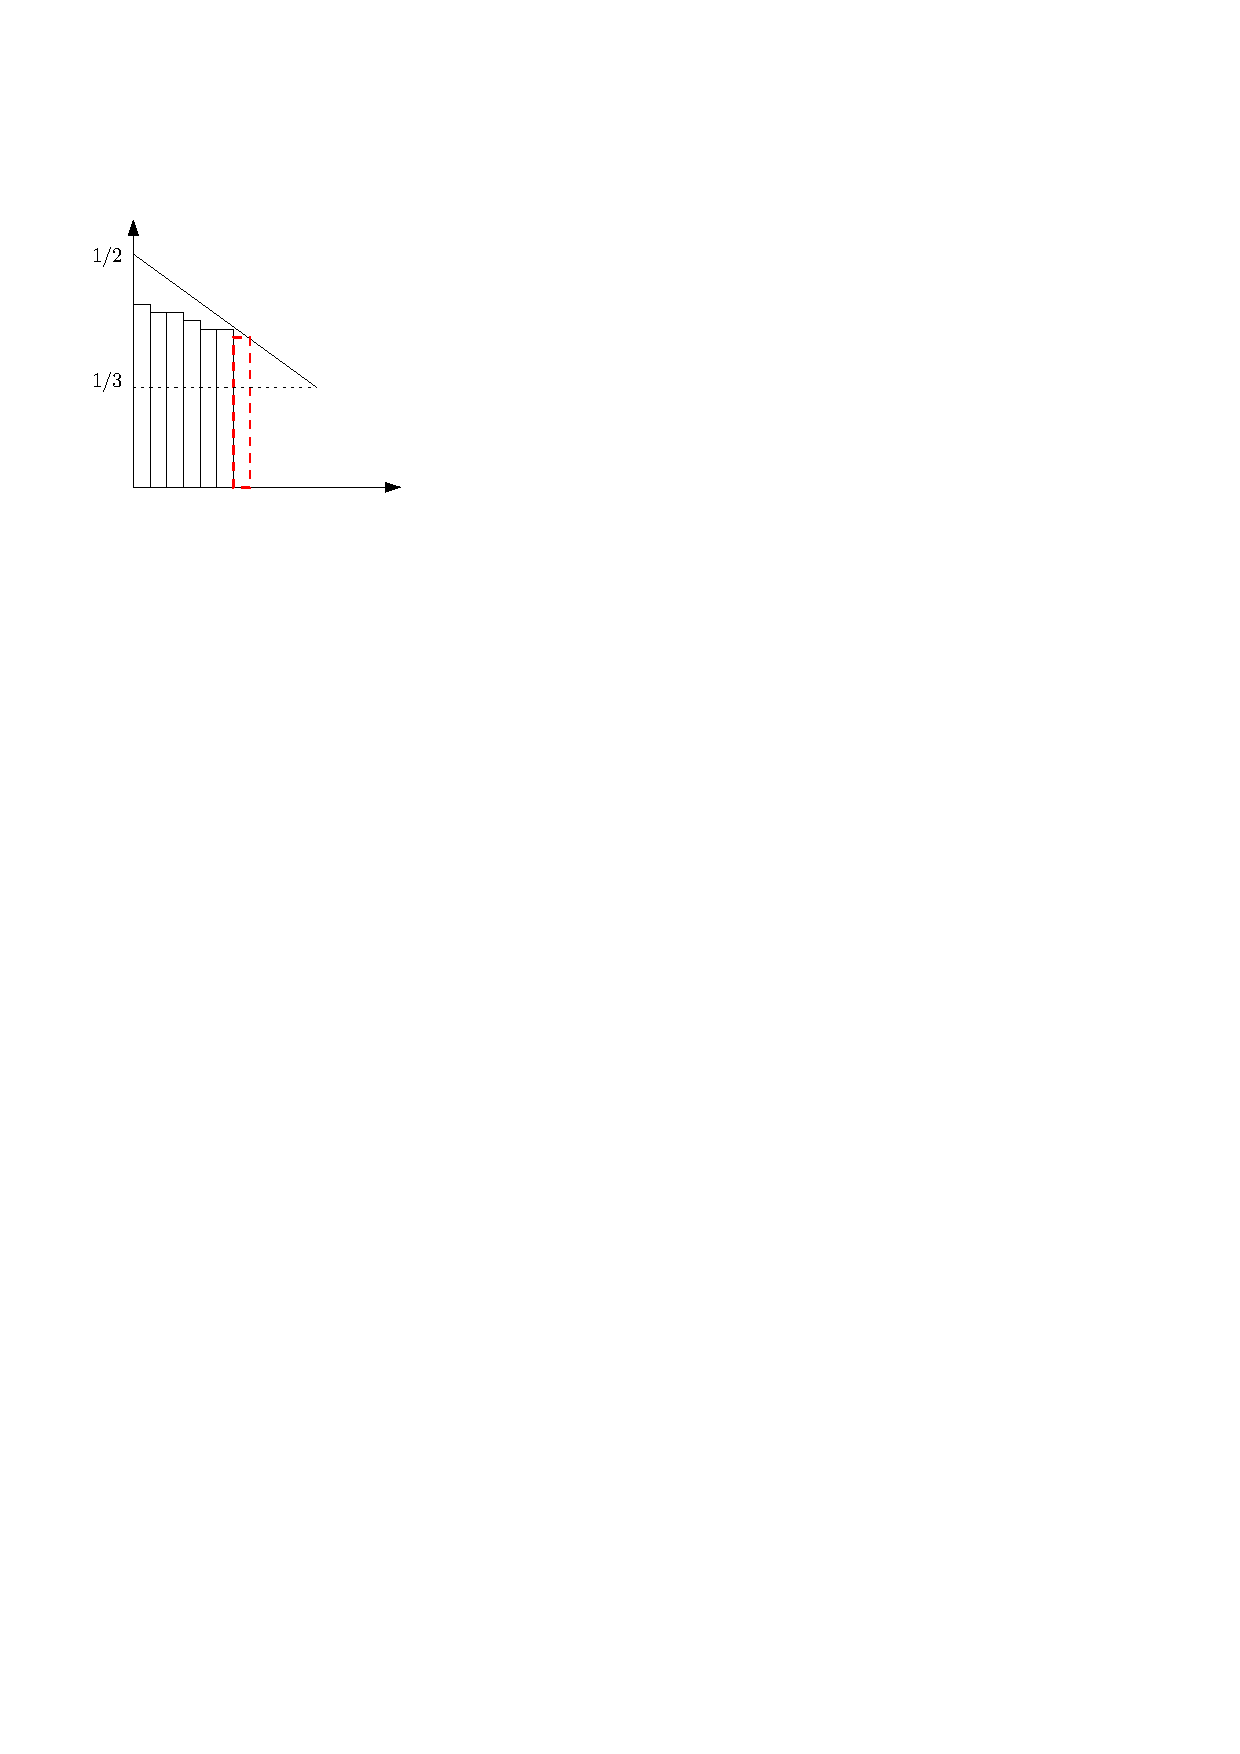
\includegraphics[width=0.5\textwidth]{figs/D_tight.pdf}
    \end{center}

    Lemat. Minimalny odrzucony $\geq$ minimalny ciasny $- O(1/n)$

    d-d. Pochodna $g$ jest ograniczona
\end{frame}


\begin{frame}{Więcej rozmiarów średnich przedmiotów}
   \begin{center}
    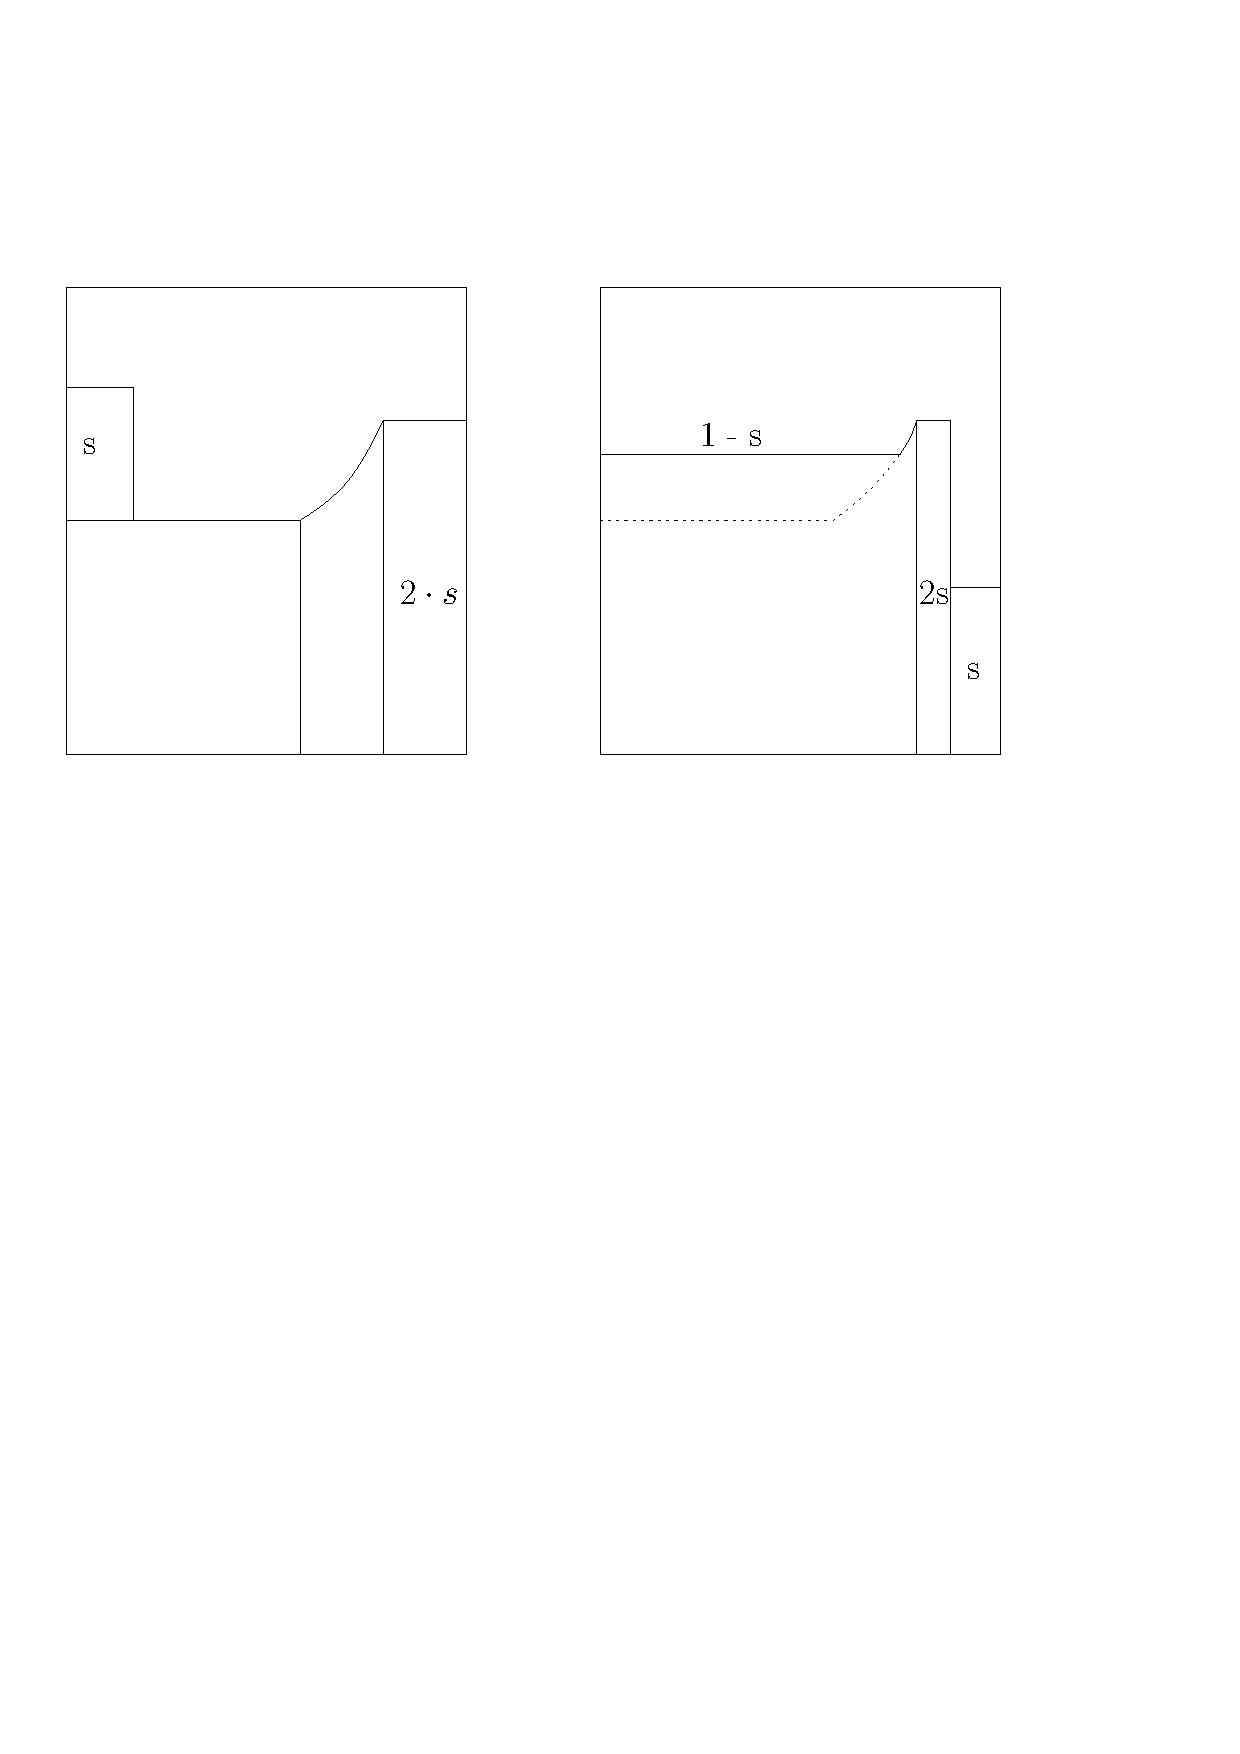
\includegraphics[width=0.8\textwidth]{figs/G1G2.pdf}
  \end{center}

  Jakie są argumenty funkcji, czyli czym jest $s$?
  
  Po lewej: $s$ to minimalny ciasny przedmiot

  Po prawej: $s$ to minimalny przedmiot
\end{frame}

\begin{frame}{Nowy przypadek w analizie}
  Minimalny ciasny może być różny niż minimalny pojedynczy. Wtedy $a$ -- minimalny ciasny, $b$ -- minimalny pojedynczy.
  
  \begin{center}
    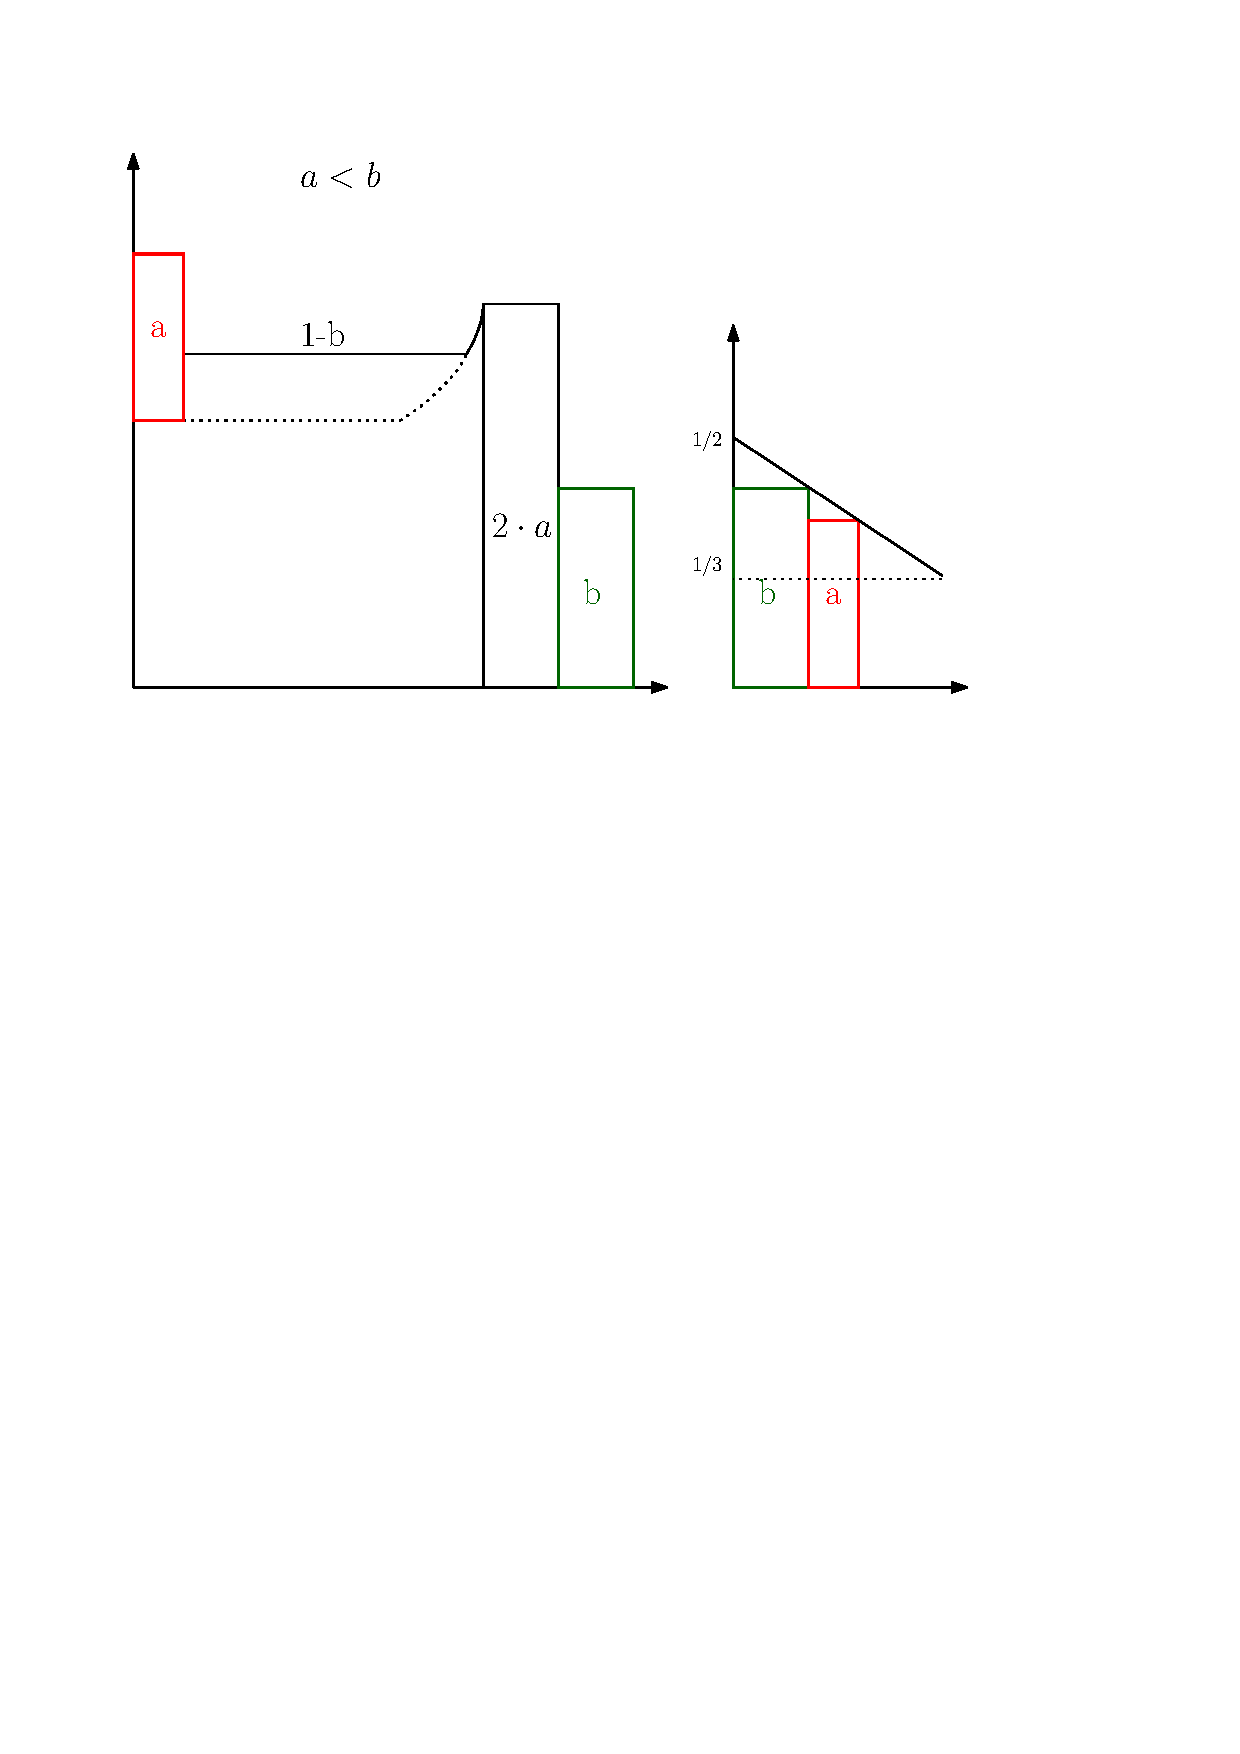
\includegraphics[width=0.8\textwidth]{figs/twoarg}
  \end{center}
  
\end{frame}

\begin{frame}{Minimalizacja funkcji dwuargumentowej}
  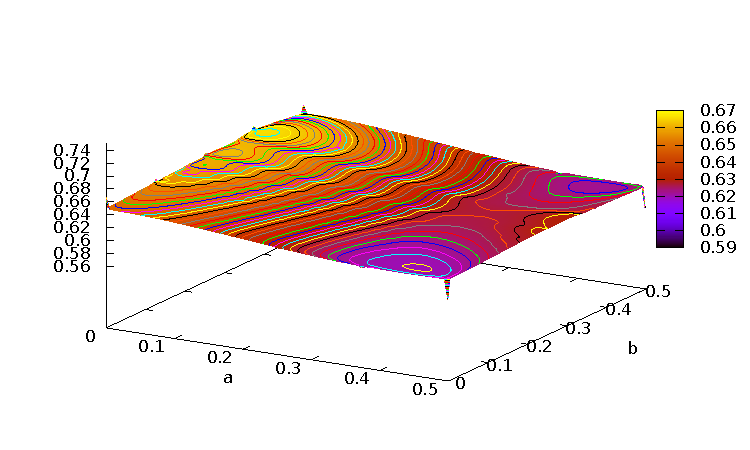
\includegraphics{figs/plot_rotated.pdf}

  \vspace{-1cm}
  \small Wykres dla $a,b \in (0, 1/2)$, choć w $0.2103\ldots$ wykres przecina się z ograniczeniem dolnym.
\end{frame}

\begin{frame}{Algorytm dla $(1/3,1]$}
  \tiny
  \begin{algorithm}[H]
  When new item $x$ arrives:\\
  \If{ there are no empty buckets left }
  {
     terminate
  }
  \If{ $x$ is large }
  {
     \If{ $x \geq f((\nBuckets(L) + \nBuckets(L^+) + 1)/n$) }
     {
  \If{ there exists any M-bucket with $x$ space left }
  {
     put $x$ in the smallest bucket with $x$ space left \hfill ($M \rightarrow L^+$)
  }
  \Else
  {
     put $x$ into any empty bucket \hfill ($\epsilon \rightarrow L$)
  }
     }
     \Else
     {
  reject
     }
  }

  \If{ x is medium }
  {
     \If{ $D\cup \{x\}$ satisfies $D$-invariant}
     {
  \If{ there exists a L-containing bucket with $x$ space left }
  {
     put $x$ in this bucket \hfill ($L \mbox{ or } L^+ \rightarrow L^+$)
  }
  \Else
  {
     put $x$ into any empty bucket \hfill ($\epsilon \rightarrow M$)
  }
     }
     \Else
     {
  \If{ there exist a $M_i$-bucket with $x$ space left}
  {
     put $x$ in this bucket \hfill ($M_* \rightarrow M_*$)
  }
  \Else
  {
     put $x$ in an empty bucket and apply $M_i$ label \hfill ($\epsilon \rightarrow M_*$)
  }
      }
  }
\end{algorithm}
\end{frame}

\end{document}